\documentclass{beamer}
\usepackage[utf8]{inputenc}
\usepackage{graphicx, epsfig}
\usepackage{amsmath,mathrsfs,amsfonts,amssymb}
\usepackage{floatflt}
\usepackage{epic,ecltree}
\usepackage{mathtext}
\usepackage{fancybox}
\usepackage{fancyhdr}
\usepackage{multirow}
\usepackage{enumerate}
\usepackage{epstopdf}
\usepackage{multicol}
\usepackage{algorithm}
\usepackage[noend]{algorithmic}
\usepackage{tikz}
\usepackage{blindtext}
\usetheme{default}%{Singapore}%{Warsaw}%{Warsaw}%{Darmstadt}
\usecolortheme{default}

\setbeamerfont{title}{size=\Huge}
\setbeamertemplate{footline}[page number]{}

\setbeamertemplate{section in toc}[sections numbered]


\makeatletter
\newcommand\HUGE{\@setfontsize\Huge{35}{40}}
\makeatother    

\setbeamerfont{title}{size=\HUGE}
\beamertemplatenavigationsymbolsempty

% latin bold lower
\newcommand{\ba}{\mathbf{a}} 
\newcommand{\bc}{\mathbf{c}} 
\newcommand{\be}{\mathbf{e}} 
\newcommand{\bh}{\mathbf{h}} 
\newcommand{\bp}{\mathbf{p}} 
\newcommand{\bt}{\mathbf{t}} 
\newcommand{\bs}{\mathbf{s}} 
\newcommand{\bu}{\mathbf{u}} 
\newcommand{\bv}{\mathbf{v}} 
\newcommand{\bw}{\mathbf{w}} 
\newcommand{\bx}{\mathbf{x}} 
\newcommand{\by}{\mathbf{y}} 
\newcommand{\bz}{\mathbf{z}} 

% latin bold upper
\newcommand{\bA}{\mathbf{A}} 
\newcommand{\bB}{\mathbf{B}} 
\newcommand{\bC}{\mathbf{C}} 
\newcommand{\bI}{\mathbf{I}} 
\newcommand{\bJ}{\mathbf{J}} 
\newcommand{\bL}{\mathbf{L}} 
\newcommand{\bM}{\mathbf{M}} 
\newcommand{\bP}{\mathbf{P}}
\newcommand{\bQ}{\mathbf{Q}} 
\newcommand{\bR}{\mathbf{R}} 
\newcommand{\bT}{\mathbf{T}} 
\newcommand{\bU}{\mathbf{U}} 
\newcommand{\bV}{\mathbf{V}} 
\newcommand{\bW}{\mathbf{W}} 
\newcommand{\bX}{\mathbf{X}} 
\newcommand{\bY}{\mathbf{Y}} 
\newcommand{\bZ}{\mathbf{Z}} 

% latin cal upper
\newcommand{\cF}{\mathcal{F}} 
\newcommand{\cG}{\mathcal{G}} 
\newcommand{\cI}{\mathcal{I}} 
\newcommand{\cL}{\mathcal{L}} 
\newcommand{\cM}{\mathcal{M}} 
\newcommand{\cN}{\mathcal{N}} 
\newcommand{\cP}{\mathcal{P}} 
\newcommand{\cS}{\mathcal{S}} 
\newcommand{\cT}{\mathcal{T}} 
\newcommand{\cW}{\mathcal{W}} 
\newcommand{\cX}{\mathcal{X}} 
\newcommand{\cZ}{\mathcal{Z}} 

% latin bb upper
\newcommand{\bbE}{\mathbb{E}} 
\newcommand{\bbI}{\mathbb{I}} 
\newcommand{\bbP}{\mathbb{P}} 
\newcommand{\bbR}{\mathbb{R}} 

% greek bold lower
\newcommand{\bepsilon}{\boldsymbol{\epsilon}} 
\newcommand{\btheta}{\boldsymbol{\theta}} 
\newcommand{\blambda}{\boldsymbol{\lambda}} 
\newcommand{\bpi}{\boldsymbol{\pi}} 
\newcommand{\bmu}{\boldsymbol{\mu}} 
\newcommand{\bsigma}{\boldsymbol{\sigma}} 
\newcommand{\bphi}{\boldsymbol{\phi}} 

% greek bold upper
\newcommand{\bSigma}{\boldsymbol{\Sigma}} 

\DeclareMathOperator*{\argmin}{arg\,min}
\DeclareMathOperator*{\argmax}{arg\,max}

\newcommand{\createdgmtitle}[1]{\title[\hbox to 56mm{Deep Generative Models  \hfill\insertframenumber\,/\,\inserttotalframenumber}]
	{\vspace{1cm} \\ \textbf{Deep Generative Models} \\ {\Huge Lecture #1}}
	\author{Roman Isachenko}
		\institute{
\includegraphics[width=0.7cm]{../utils/aimasterslogo} \LARGE{AI Masters}}
	\date{2024, Spring}
}

\usepackage{tikz}
\usetikzlibrary{arrows,shapes,positioning,shadows,trees}

\newcommand\myfootnote[1]{%
  \tikz[remember picture,overlay]
  \draw (current page.south west) +(1in + \oddsidemargin,0.5em)
  node[anchor=south west,inner sep=0pt]{\parbox{\textwidth}{%
      \rlap{\rule{10em}{0.4pt}}\raggedright\scriptsize \textit{#1}}};}

\newcommand\myfootnotewithlink[2]{%
  \tikz[remember picture,overlay]
  \draw (current page.south west) +(1in + \oddsidemargin,0.5em)
  node[anchor=south west,inner sep=0pt]{\parbox{\textwidth}{%
      \rlap{\rule{10em}{0.4pt}}\raggedright\scriptsize\href{#1}{\textit{#2}}}};}
      
\AtBeginSection[]
      {
      	\begin{frame}{Outline}
      		\tableofcontents[currentsection]
      	\end{frame}
      }
      \AtBeginSubsection[]{
      	\begin{frame}{Outline}
      		\tableofcontents[currentsection,currentsubsection]
      	\end{frame}
}
\createdgmtitle{6}
%--------------------------------------------------------------------------------
\begin{document}
%--------------------------------------------------------------------------------
\begin{frame}[noframenumbering,plain]
%\thispagestyle{empty}
\titlepage
\end{frame}
%=======
\begin{frame}{Recap of previous lecture}
	\begin{block}{EM-algorithm}
	\begin{itemize}
		\item E-step
		\[
			q^*(\bz) = \argmax_q \mathcal{L} (q, \btheta^*)
			= \argmin_q KL(q(\bz) || p(\bz | \bx, \btheta^*));
		\]
		\item M-step
		\[
			\btheta^* = \argmax_{\btheta} \mathcal{L} (q^*, \btheta);
		\]
	\end{itemize}
	\vspace{-0.3cm}
	\end{block}
	\begin{block}{Amortized variational inference}
	Restrict a family of all possible distributions $q(\bz)$ to a parametric class $q(\bz|\bx, \bphi)$ conditioned on samples $\bx$ with parameters $\bphi$.
	\end{block}
	
	\textbf{Variational Bayes}
	\begin{itemize}
		\item E-step
		\[
		\bphi_k = \bphi_{k-1} + \left.\eta \cdot \nabla_{\bphi} \mathcal{L}(\bphi, \btheta_{k-1})\right|_{\bphi=\bphi_{k-1}}
		\]
		\item M-step
		\[
		\btheta_k = \btheta_{k-1} + \left.\eta \cdot \nabla_{\btheta} \mathcal{L}(\bphi_k, \btheta)\right|_{\btheta=\btheta_{k-1}}
		\]
	\end{itemize}
\end{frame}
%=======
\begin{frame}{Recap of previous lecture}
	\vspace{-0.3cm}
	\[
		 \mathcal{L} (\bphi, \btheta)  = \mathbb{E}_{q(\bz | \bx, \bphi)} \left[\log p(\bx | \bz, \btheta) - \log \frac{q(\bz | \bx, \bphi)}{p(\bz)} \right] \rightarrow \max_{\bphi, \btheta}.
	\]	
	\vspace{-0.3cm}
	\begin{block}{M-step: $\nabla_{\btheta} \mathcal{L}(\bphi, \btheta)$, Monte Carlo estimation}
		\vspace{-0.8cm}
		\begin{multline*}
			\nabla_{\btheta} \mathcal{L} (\bphi, \btheta)
			= \int q(\bz|\bx, \bphi) \nabla_{\btheta}\log p(\bx|\bz, \btheta) d \bz \approx  \\
			\approx \nabla_{\btheta}\log p(\bx|\bz^*, \btheta), \quad \bz^* \sim q(\bz|\bx, \bphi).
		\end{multline*}
		\vspace{-0.7cm}
	\end{block}
	\begin{block}{E-step: $\nabla_{\bphi} \mathcal{L}(\bphi, \btheta)$, reparametrization trick}
		\vspace{-0.8cm}
		\begin{multline*}
			\nabla_{\bphi} \mathcal{L} (\bphi, \btheta) = \int r(\bepsilon) \nabla_{\bphi} \log p(\bx | \bg_{\bphi}(\bx, \bepsilon), \btheta) d\bepsilon  - \nabla_{\bphi} \text{KL}
			\\ \approx \nabla_{\bphi} \log p(\bx | \bg_{\bphi}(\bx, \bepsilon^*), \btheta)  - \nabla_{\bphi} \text{KL}
		\end{multline*}
		\vspace{-0.5cm}
	\end{block}
	\vspace{-0.5cm}
	
	\begin{block}{Variational assumption}
		\vspace{-0.3cm}
		\[
			r(\bepsilon) = \mathcal{N}(0, \bI); \quad  q(\bz| \bx, \bphi) = \mathcal{N} (\bmu_{\bphi}(\bx), \bsigma^2_{\bphi}(\bx)).
		\]
		\[
			\bz = \bg_{\bphi}(\bx, \bepsilon) = \bsigma_{\bphi}(\bx) \odot \bepsilon + \bmu_{\bphi}(\bx).
		\]
	\end{block}
\end{frame}
%=======
\begin{frame}{Recap of previous lecture}
	\begin{block}{Final EM-algorithm}
		\begin{itemize}
			\item pick random sample $\bx_i, i \sim U[1, n]$.
			\item compute the objective:
			\vspace{-0.3cm}
			\[
			\bepsilon^* \sim r(\bepsilon); \quad \bz^* = \bg_{\bphi}(\bx, \bepsilon^*);
			\]
			\[
			\cL(\bphi, \btheta) \approx  \log p(\bx | \bz^*, \btheta) - KL(q(\bz^* | \bx, \bphi) || p(\bz^*)).
			\]
			\item compute a stochastic gradients w.r.t. $\bphi$ and $\btheta$
			\begin{align*}
				\nabla_{\bphi} \mathcal{L} (\bphi, \btheta) &\approx \nabla_{\bphi} \log p(\bx | \bg_{\bphi}(\bx, \bepsilon^*), \btheta)  - \nabla_{\bphi} \text{KL}(q(\bz | \bx, \bphi) || p(\bz)); \\
				\nabla_{\btheta} \mathcal{L} (\bphi, \btheta) &\approx \nabla_{\btheta} \log p(\bx|\bz^*, \btheta).
			\end{align*}
			\item update $\btheta, \bphi$ according to the selected optimization method (SGD, Adam):
			\begin{align*}
				\bphi &:= \bphi + \eta \cdot \nabla_{\bphi} \mathcal{L}(\bphi, \btheta), \\
				\btheta &:= \btheta + \eta \cdot \nabla_{\btheta} \mathcal{L}(\bphi, \btheta).
			\end{align*}
		\end{itemize}
	\end{block}
\end{frame}
%=======
\begin{frame}{Recap of previous lecture}
	\begin{minipage}[t]{0.55\columnwidth}
		\begin{block}{Variational autoencoder (VAE)}
		    \begin{itemize}
			    \item VAE learns stochastic mapping between $\bx$-space, from $\pi(\bx)$, and a latent $\bz$-space, with simple distribution. 
			    \item The generative model learns  distribution $p(\bx, \bz | \btheta) = p(\bz) p(\bx |\bz, \btheta)$, with a prior distribution $p(\bz)$, and a stochastic decoder $p(\bx|\bz, \btheta)$. 
			    \item The stochastic encoder $q(\bz|\bx, \bphi)$ (inference model), approximates the true but intractable posterior $p(\bz|\bx, \btheta)$.
		    \end{itemize}
	    \end{block}
	\end{minipage}%
	\begin{minipage}[t]{0.45\columnwidth}
		\vspace{0.7cm}
		\begin{figure}[h]
			\centering
			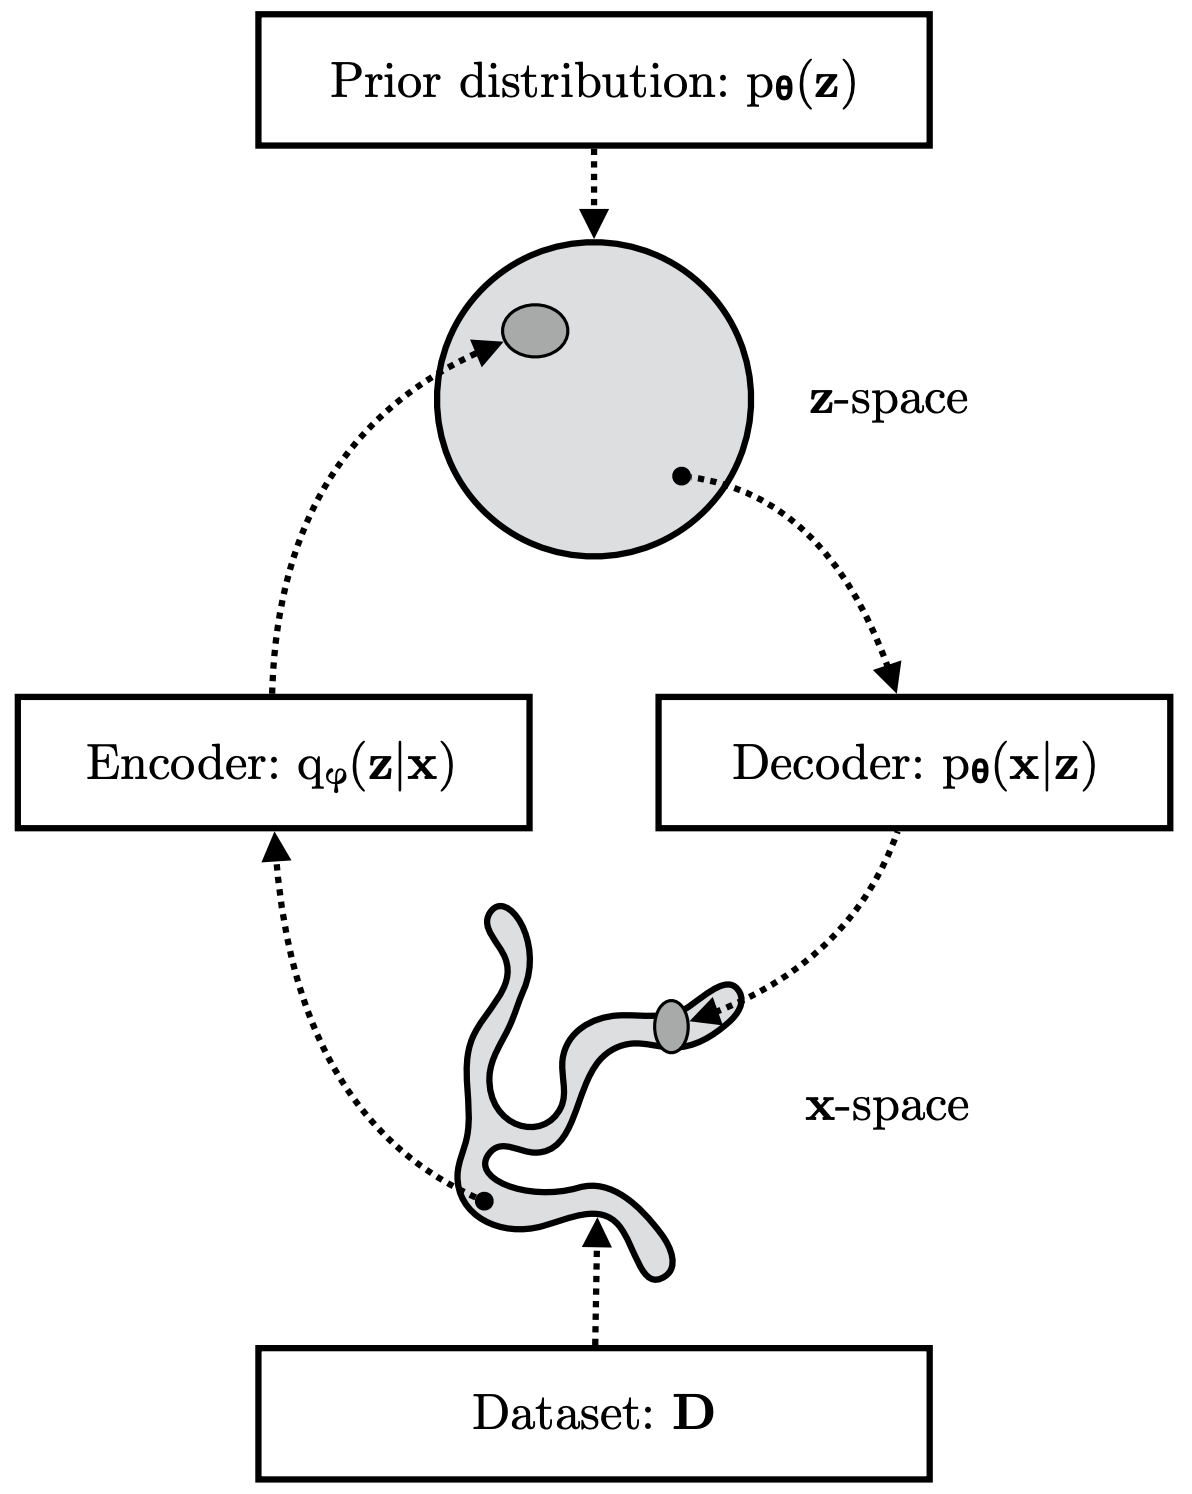
\includegraphics[width=\linewidth]{figs/vae_scheme}
		\end{figure}
	\end{minipage}
	
	\myfootnotewithlink{https://arxiv.org/abs/1906.02691}{Kingma D. P., Welling M. An introduction to variational autoencoders, 2019}
\end{frame}
%=======
\begin{frame}{Recap of previous lecture}
	\begin{table}[]
		\begin{tabular}{l|c|c}
			& \textbf{VAE} & \textbf{NF} \\ \hline
			\textbf{Objective} & ELBO $\cL$ & Forward KL/MLE \\ \hline
			\textbf{Encoder} & \shortstack{stochastic \\ $\bz \sim q (\bz | \bx, \bphi)$} &  \shortstack{\\ deterministic \\ $\bz = \bff_{\btheta}(\bx)$ \\ $q(\bz | \bx, \btheta) = \delta(\bz - \bff_{\btheta}(\bx))$}  \\ \hline
			\textbf{Decoder} & \shortstack{stochastic \\ $\bx \sim p (\bx | \bz, \btheta)$} & \shortstack{\\ deterministic \\ $\bx = \bg_{\btheta}(\bz)$ \\ $ p(\bx | \bz, \btheta) = \delta(\bx - \bg_{\btheta}(\bz))$} \\ \hline
			\textbf{Parameters}  & $\bphi, \btheta$ & $\btheta \equiv \bphi$\\ 
		\end{tabular}
	\end{table}
	\begin{block}{Theorem}
		MLE for normalizing flow is equivalent to maximization of ELBO for VAE model with deterministic encoder and decoder:
		\vspace{-0.3cm}
		\[
		p(\bx | \bz, \btheta) = \delta (\bx - \bff^{-1}_{\btheta}(\bz)) = \delta (\bx - \bg_{\btheta}(\bz));
		\]
		\[
		q(\bz | \bx, \btheta) = p(\bz | \bx, \btheta) = \delta (\bz - \bff_{\btheta}(\bx)).
		\]
	\end{block}
	\myfootnotewithlink{https://arxiv.org/abs/2007.02731}{Nielsen D., et al. SurVAE Flows: Surjections to Bridge the Gap between VAEs and Flows, 2020}
\end{frame}
%=======
\section{Discrete VAE latent representations}
%=======
\begin{frame}{Discrete VAE latents}
	\begin{block}{Motivation}
		\begin{itemize}
			\item Previous VAE models had \textbf{continuous} latent variables $\bz$.
			\item \textbf{Discrete} representations $\bz$ are potentially a more natural fit for many of the modalities.
			\item Powerful autoregressive models (like PixelCNN) have been developed for modelling distributions over discrete variables.
			\item All cool transformer-like models work with discrete tokens.
		\end{itemize}
	\end{block}
	\begin{block}{ELBO}
		\vspace{-0.3cm}
		\[
		\mathcal{L} (\bphi, \btheta)  = \mathbb{E}_{q(\bz | \bx, \bphi)} \log p(\bx | \bz , \btheta) - KL(q(\bz| \bx, \bphi) || p(\bz)) \rightarrow \max_{\bphi, \btheta}.
		\]
		\vspace{-0.5cm}
	\end{block}
	\begin{itemize}
		\item Reparametrization trick to get unbiased gradients.
		\item Normal assumptions for $q(\bz | \bx, \bphi)$ and $p(\bz)$ to compute KL analytically.
	\end{itemize}
\end{frame}
%=======
\begin{frame}{Discrete VAE latents}
	\begin{block}{Assumptions}
		\begin{itemize}
			\item Let $c \sim \text{Categorical}(\bpi)$, where 
			\vspace{-0.6cm}
			\[
			\bpi = (\pi_1, \dots, \pi_K), \quad \pi_k = P(c = k), \quad \sum_{k=1}^K \pi_k = 1.
			\]
			\vspace{-0.6cm}
			\item Let VAE model has discrete latent representation $c$ with prior $p(c) = \text{Uniform}\{1, \dots, K\}$.
		\end{itemize}
	\end{block}
	\begin{block}{ELBO}
		\vspace{-0.5cm}
		\[
			\mathcal{L} (\bphi, \btheta)  = \mathbb{E}_{q(c | \bx, \bphi)} \log p(\bx | c, \btheta) - {\color{olive} KL(q(c| \bx, \bphi) || p(c))} \rightarrow \max_{\bphi, \btheta}.
		\]
	\end{block}
	\vspace{-1.0cm}
	{\small
	\begin{multline*}
		{\color{olive} KL(q(c| \bx, \bphi) || p(c))} = \sum_{k=1}^K q(k | \bx, \bphi) \log \frac{q(k | \bx, \bphi)}{p(k)} = 
		\\ = \color{violet}{\sum_{k=1}^K q(k | \bx, \bphi) \log q(k | \bx, \bphi)}  \color{teal}{- \sum_{k=1}^K q(k | \bx, \bphi) \log p(k)}  = \\ = \color{violet}{- H(q(c | \bx, \bphi))} + \color{teal}{\log K}. 
	\end{multline*}
	}
\end{frame}
%=======
\begin{frame}{Discrete VAE latents}
	\vspace{-0.3cm}
	\[
		\mathcal{L} (\bphi, \btheta)  = \mathbb{E}_{q(c | \bx, \bphi)} \log p(\bx | c, \btheta) + H(q(c | \bx, \bphi)) - \log K \rightarrow \max_{\bphi, \btheta}.
	\]
	\vspace{-0.3cm}
	\begin{itemize}
		\item Our encoder should output discrete distribution $q(c | \bx, \bphi)$.
		\item We need the analogue of the reparametrization trick for the discrete distribution $q(c | \bx, \bphi)$.
		\item Our decoder $p(\bx | c, \btheta)$ should input discrete random variable $c$.
	\end{itemize}
	\begin{figure}[h]
		\centering
		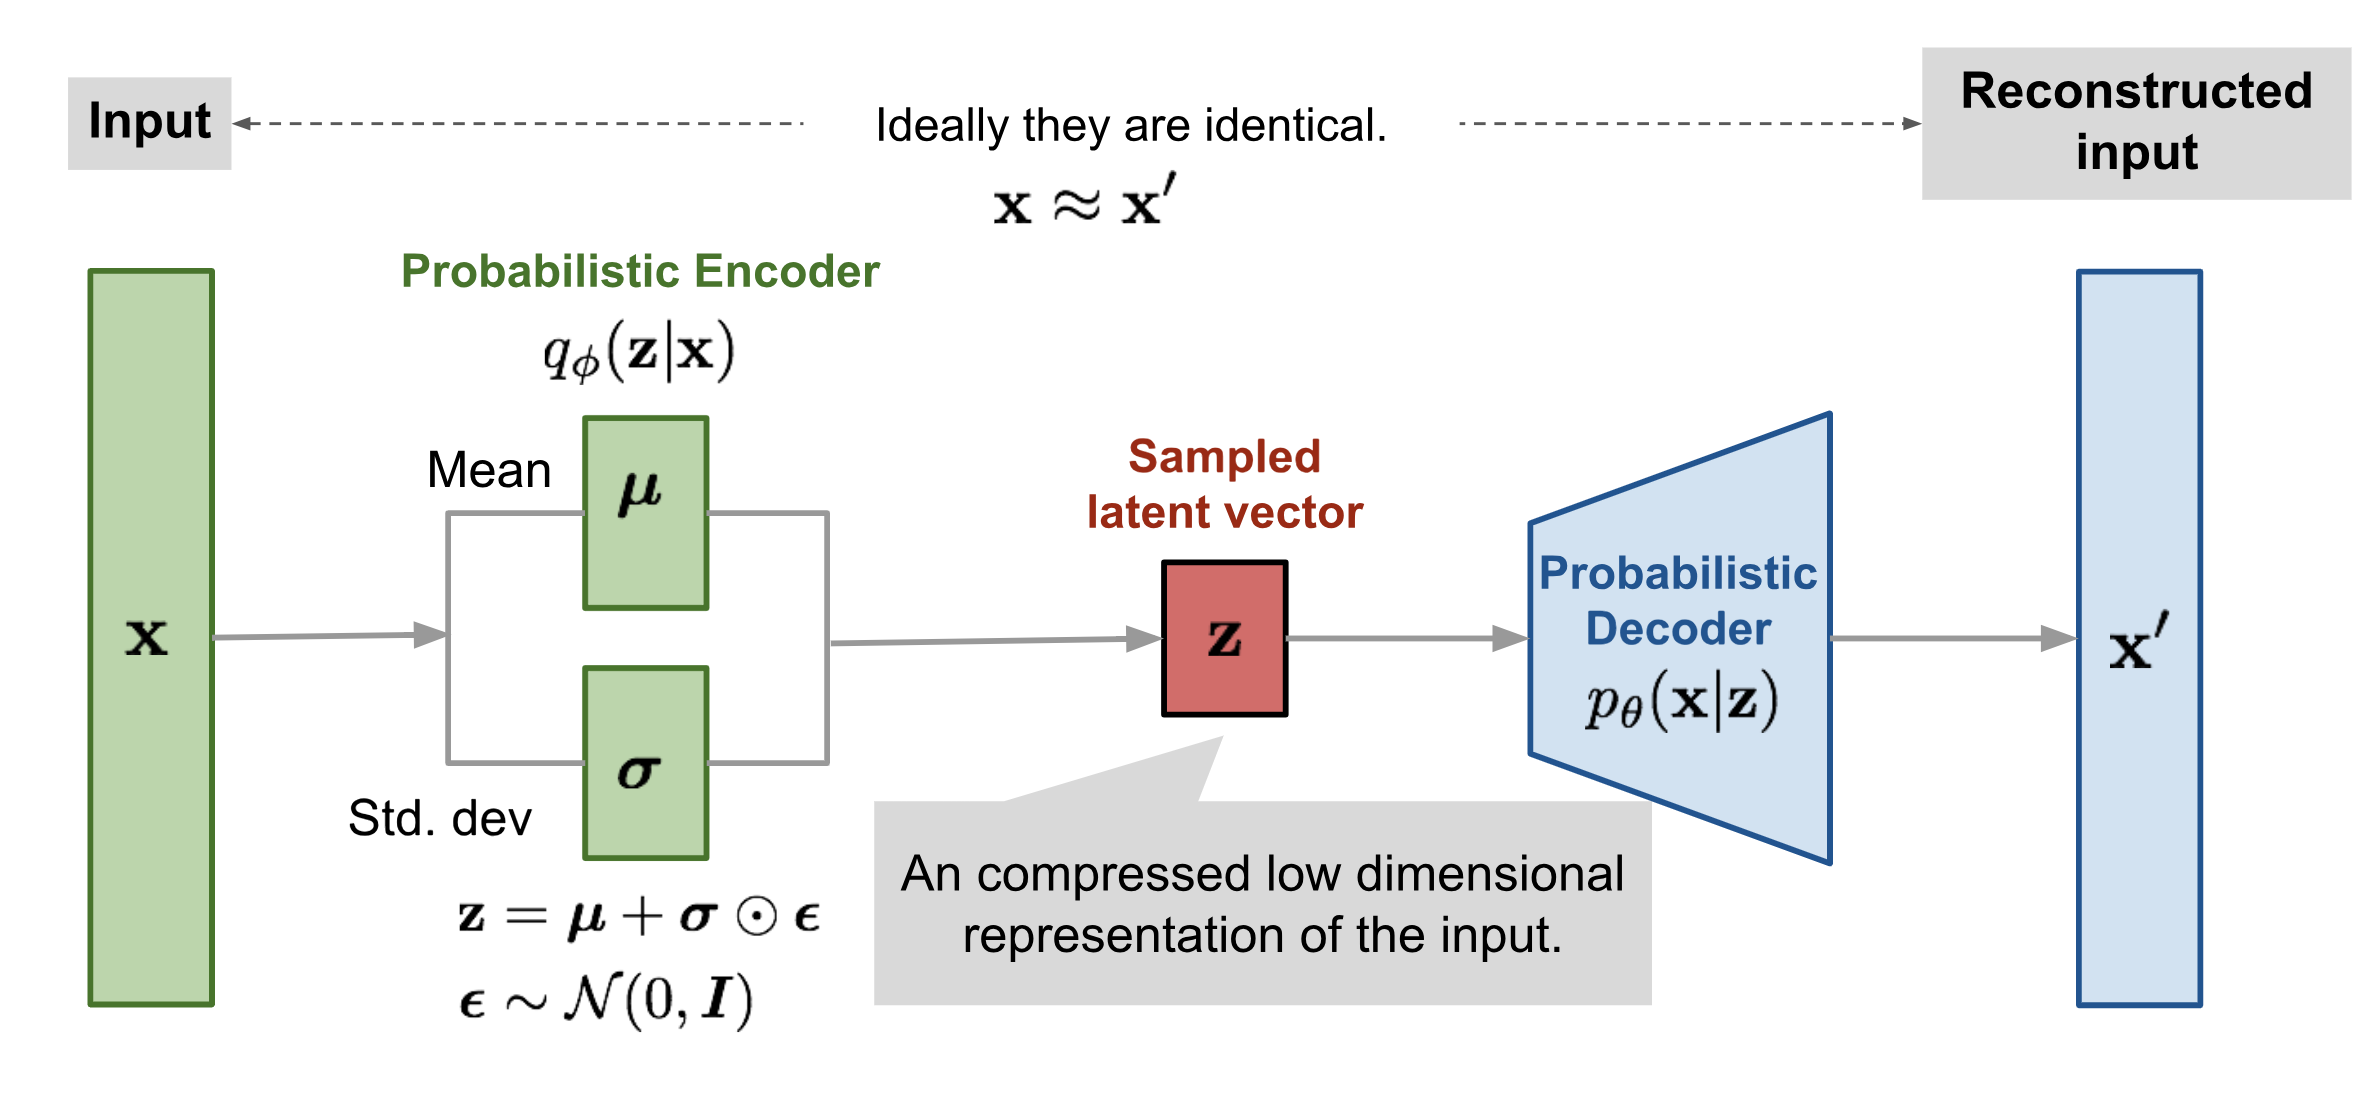
\includegraphics[width=0.9\linewidth]{figs/vae-gaussian}
	\end{figure}
	\myfootnotewithlink{https://lilianweng.github.io/lil-log/2018/08/12/from-autoencoder-to-beta-vae.html}{image credit: https://lilianweng.github.io/lil-log/2018/08/12/from-autoencoder-to-beta-vae.html}
\end{frame}
%=======
\subsection{Vector quantization}
%=======
\begin{frame}{Discrete VAE latents}
	\begin{block}{How to implement this model?}
		\begin{itemize}
			\item Variational posterior $q(c | \bx, \bphi) = \text{Categorical}(\bpi_{\bphi}(\bx))$ (encoder) outputs discrete probabilities vector.
			\item We sample $c^*$ from $q(c | \bx, \bphi)$ (reparametrization trick analogue).
			\item Define the dictionary space $\{\be_k\}_{k=1}^K$, where $\be_k \in \bbR^C$, $K$ is the size of the dictionary.
			\item We use $\be_{c^*}$ in the generative distribution $p(\bx | \be_{c^*}, \btheta)$ (decoder).
		\end{itemize}
	\end{block}
\end{frame}
%=======
\begin{frame}{Vector quantization}
	Define the dictionary space $\{\be_k\}_{k=1}^K$, where $\be_k \in \bbR^C$, $K$ is the size of the dictionary.
	\begin{block}{Quantized representation}
		$\bz_q \in \bbR^{C}$  for $\bz \in \bbR^C$ is defined by a nearest neighbor look-up using the  dictionary space
		\vspace{-0.3cm}
		\[
		\bz_q = \bq (\bz) = \be_{k^*}, \quad \text{where } k^* = \argmin_k \| \bz - \be_k \|.
		\] 
		\vspace{-0.7cm}
	\end{block}
	\vspace{-0.2cm}
	\begin{block}{Quantization procedure}
		If we have tensor with the spatial dimensions we apply the quantization for each of $W \times H$ locations.
		\begin{minipage}[t]{0.65\columnwidth}
			\begin{figure}
				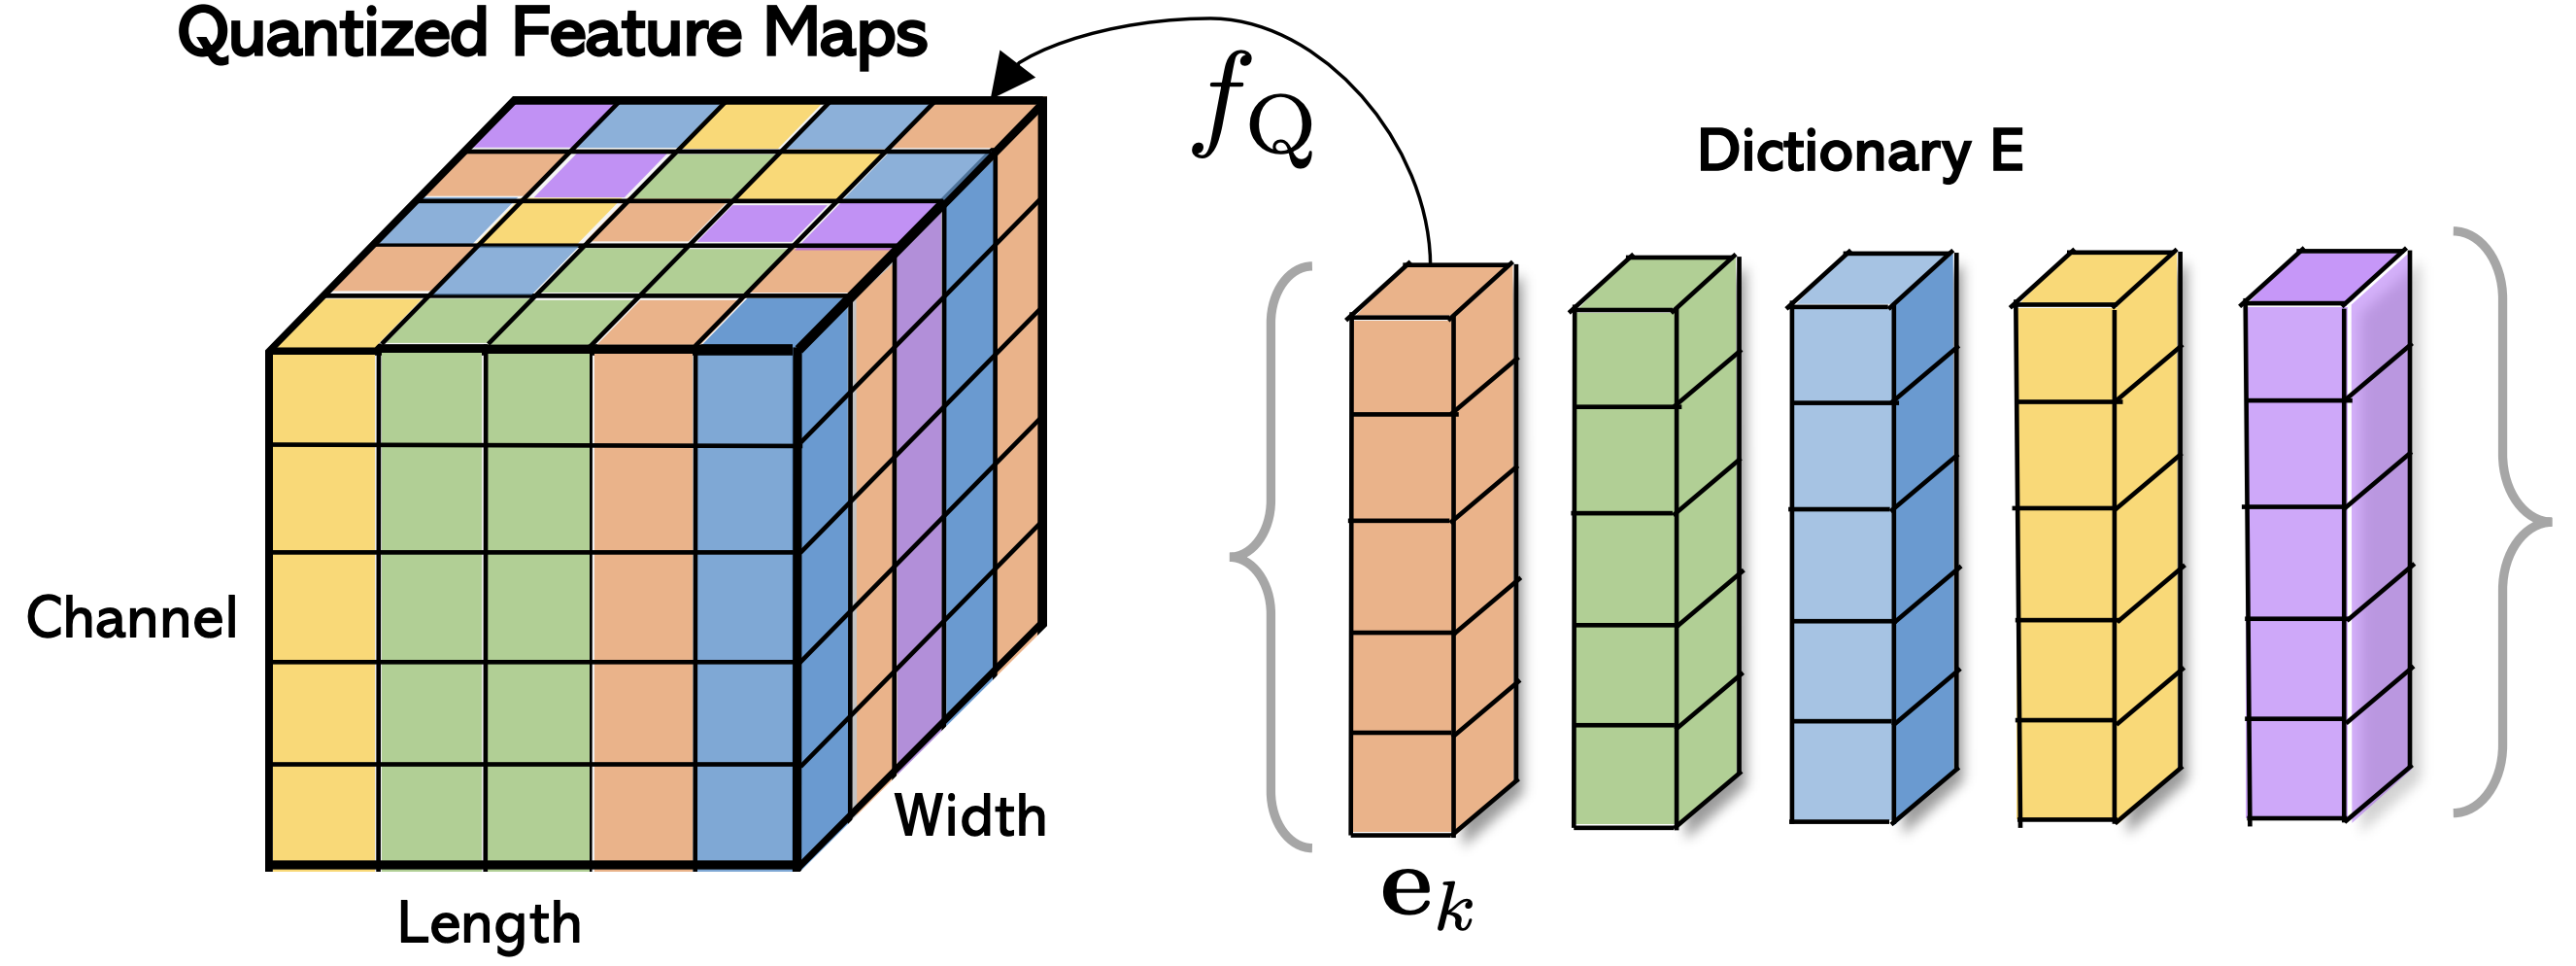
\includegraphics[width=0.8\linewidth]{figs/fqgan_cnn.png}
			\end{figure}
		\end{minipage}%
		\begin{minipage}[t]{0.35\columnwidth}
			\begin{figure}
				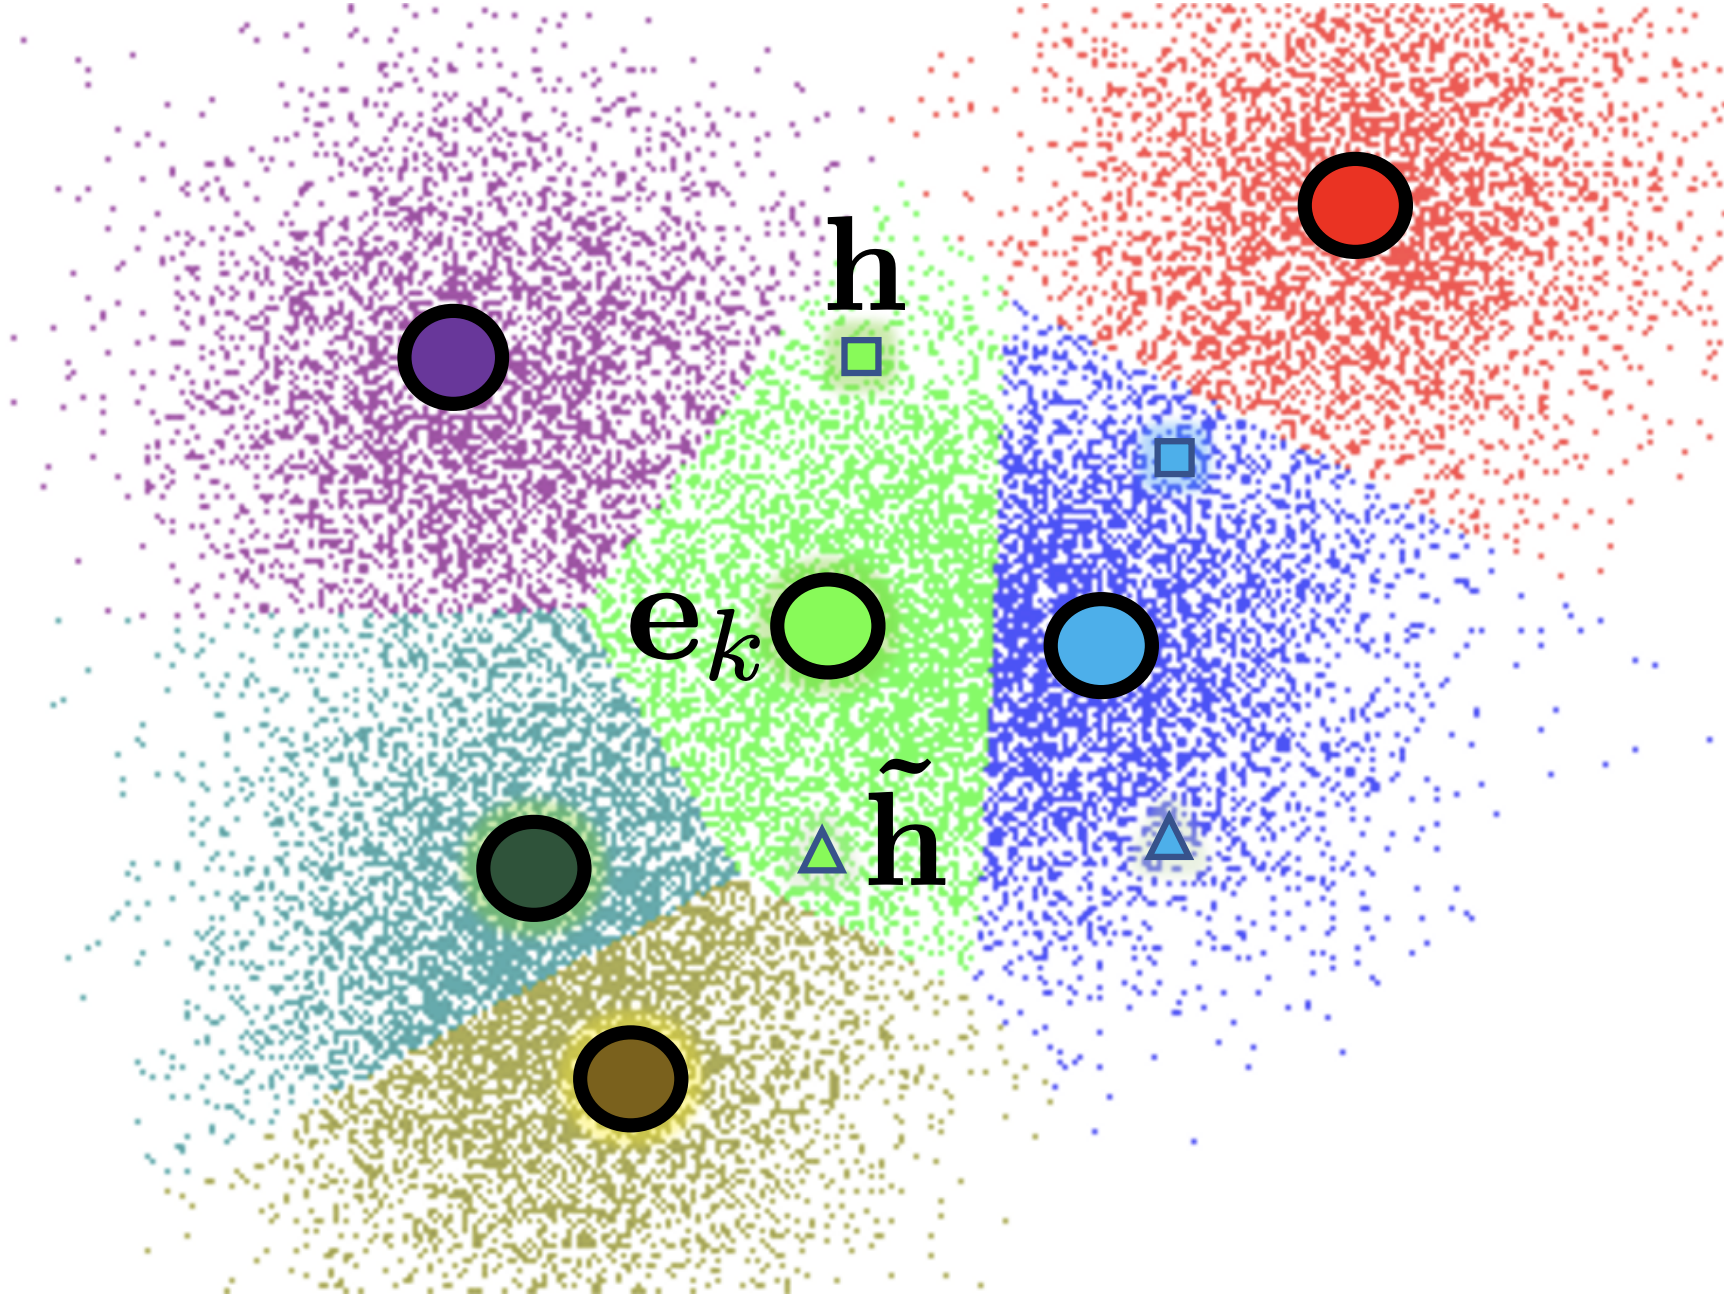
\includegraphics[width=0.7\linewidth]{figs/fqgan_lookup}
			\end{figure}
		\end{minipage}
	\end{block}
	\myfootnotewithlink{https://arxiv.org/abs/2004.02088}{Zhao Y. et al. Feature Quantization Improves GAN Training, 2020} 
\end{frame}
%=======
\begin{frame}{Vector Quantized VAE (VQ-VAE)}
	\begin{itemize}
		\item Let our encoder outputs continuous representation $\bz_e = \text{NN}_{e, \bphi}(\bx) \in \bbR^{C}$.
		\item Quantization will give us the deterministic mapping from the encoder output $\bz_e$ to its quantized representation $\bz_q$.
		\item Let use the dictionary elements $\be_c$ in the generative distribution $p(\bx | \be_c, \btheta)$ (decoder).
	\end{itemize}
	\begin{block}{Deterministic variational posterior}
		\vspace{-0.3cm}
		\[
			q(c = k^* | \bx, \bphi) = \begin{cases}
				1 , \quad \text{for } k^* = \argmin_k \| \bz_e - \be_k \|; \\
				0, \quad \text{otherwise}.
		\end{cases}
		\]
		\[
			KL(q(c | \bx, \bphi) || p(c)) = - \underbrace{H(q(c | \bx, \bphi))}_{=0} + \log K = \log K. 
		\]
	\end{block}	
	\vspace{-0.4cm}
	Generalization to the spatial dimension: $\bc \in \{1, \dots, K\}^{W \times H}$
	\[
		q(\bc | \bx, \bphi) = \prod_{i=1}^W \prod_{j=1}^H q(c_{ij} | \bx, \bphi); \quad p(\bc) = \prod_{i=1}^W \prod_{j=1}^H \text{Uniform}\{1, \dots, K\}.
	\]
	\myfootnotewithlink{https://arxiv.org/abs/1711.00937}{Oord A., Vinyals O., Kavukcuoglu K. Neural Discrete Representation Learning, 2017} 
\end{frame}
%=======
\begin{frame}{Vector Quantized VAE (VQ-VAE)}
	\begin{block}{ELBO}
		\vspace{-0.6cm}
		\[
		\mathcal{L} (\bphi, \btheta)  = \mathbb{E}_{q(c | \bx, \bphi)} \log p(\bx | \be_{c} , \btheta) - \log K =  \log p(\bx | \bz_q, \btheta) - \log K,
		\]
		where $\bz_q = \be_{k^*}$, $k^* = \argmin_k \| \bz_e - \be_k \|$.
	\end{block}
	\begin{figure}
		\centering
		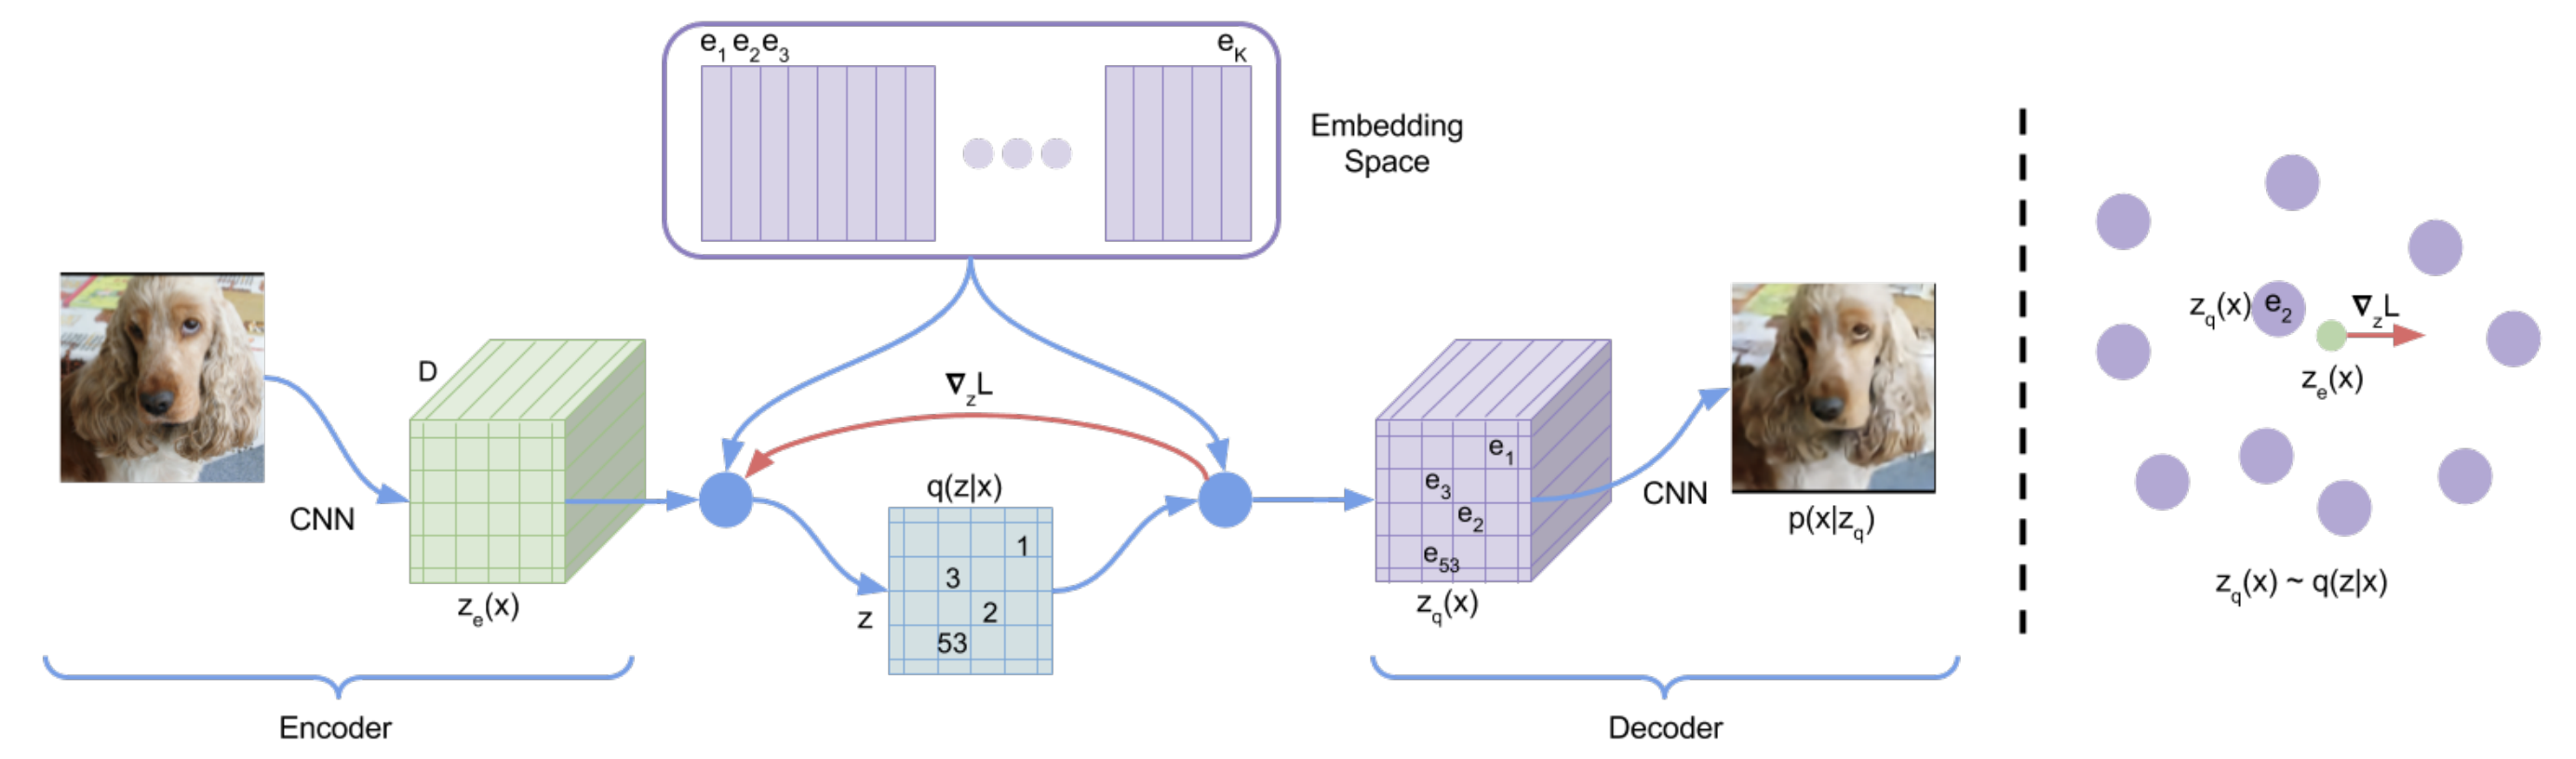
\includegraphics[width=0.85\linewidth]{figs/vqvae}
	\end{figure}
	\textbf{Problem:} $\argmin$ is not differentiable.
	\begin{block}{Straight-through gradient estimation}
		\vspace{-0.6cm}
		\[
		\frac{\partial \log p(\bx | \bz_q , \btheta)}{\partial \bphi} = \frac{\partial \log p(\bx | \bz_q, \btheta)}{\partial \bz_q} \cdot {\color{red}\frac{\partial \bz_q}{\partial \bphi}} \approx \frac{\partial \log p(\bx | \bz_q, \btheta)}{\partial \bz_q} \cdot \frac{\partial \bz_e}{\partial \bphi}
		\]
	\end{block}
	\myfootnotewithlink{https://arxiv.org/abs/1711.00937}{Oord A., Vinyals O., Kavukcuoglu K. Neural Discrete Representation Learning, 2017} 
\end{frame}
%=======
\begin{frame}{Vector Quantized VAE-2  (VQ-VAE-2)}
	\begin{block}{Samples 1024x1024}
		\vspace{-0.2cm}
		\begin{figure}
			\centering
			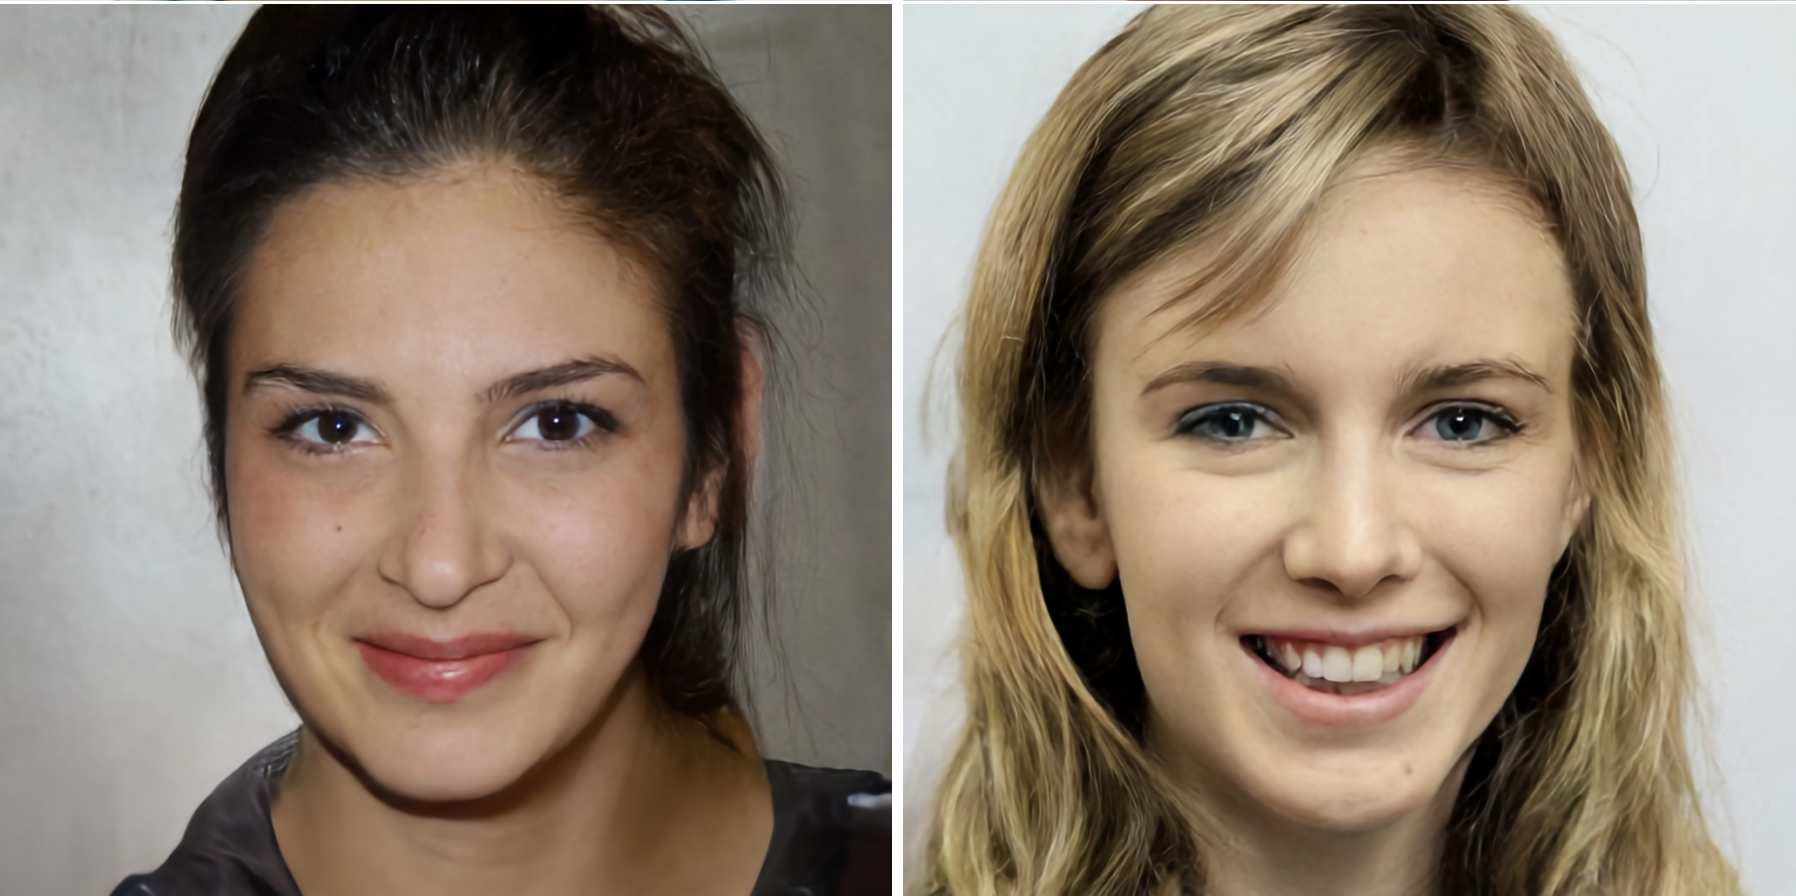
\includegraphics[width=0.63\linewidth]{figs/vqvae2_faces}
		\end{figure}
	\end{block}
	\vspace{-0.6cm}
	\begin{block}{Samples diversity}
		\vspace{-0.2cm}
		\begin{figure}
			\centering
			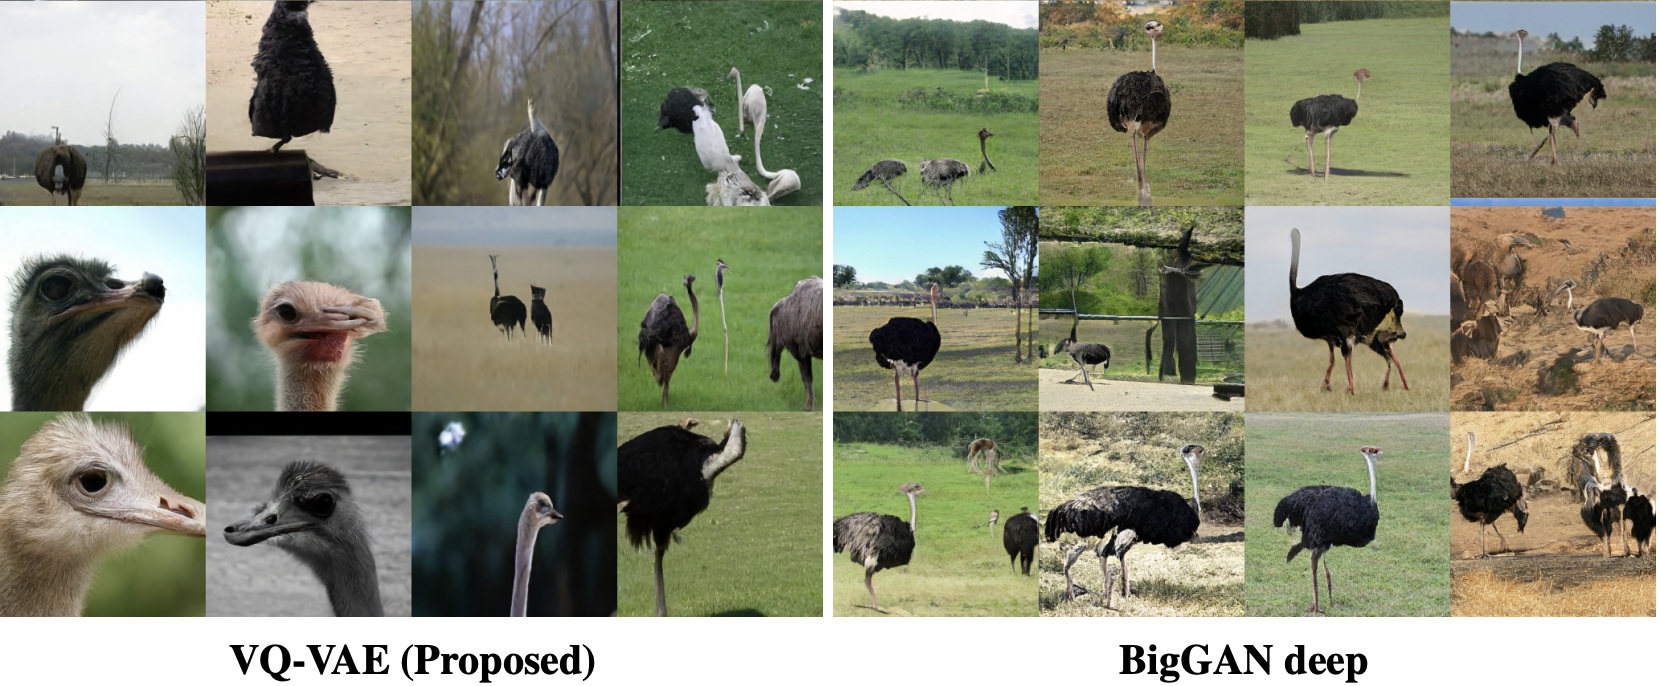
\includegraphics[width=0.65\linewidth]{figs/vqvae2_diversity}
		\end{figure}
	\end{block}
	\myfootnotewithlink{https://arxiv.org/abs/1906.00446}{Razavi A., Oord A., Vinyals O. Generating Diverse High-Fidelity Images with VQ-VAE-2, 2019} 
\end{frame}
%=======
\subsection{Gumbel-softmax for discrete VAE latents}
%=======
\begin{frame}{Gumbel-softmax trick}
	\begin{itemize}
		\item VQ-VAE has deterministic variational posterior (it allows to get rid of discrete sampling and reparametrization trick).
		\item There is no uncertainty in the encoder output. 
	\end{itemize}
	\vspace{-0.2cm}
	\begin{block}{Gumbel-max trick}
		Let $g_k \sim \text{Gumbel}(0, 1)$ for $k = 1, \dots, K$, i.e. $g = - \log (- \log u)$, $u \sim \text{Uniform}[0, 1]$. Then a discrete random variable
		\vspace{-0.2cm}
		\[
			c = \argmax_k [\log \pi_k + g_k],
		\]
		\vspace{-0.5cm} \\
		has a categorical distribution $c \sim \text{Categorical}(\bpi)$.
	\end{block}
	\begin{itemize}
		\item Let our encoder $q(c | \bx, \bphi) = \text{Categorical}(\bpi_{\bphi}(\bx))$ outputs logits of $\bpi_{\bphi}(\bx)$.
		\item We could sample from the discrete distribution using Gumbel-max reparametrization.
	\end{itemize}

	\myfootnote{
	\href{https://arxiv.org/abs/1611.00712}{Maddison C. J., Mnih A., Teh Y. W. The Concrete distribution: A continuous relaxation of discrete random variables, 2016} \\
	\href{https://arxiv.org/abs/1611.01144}{Jang E., Gu S., Poole B. Categorical reparameterization with Gumbel-Softmax, 2016}
	}
\end{frame}
%=======
\begin{frame}{Gumbel-softmax trick}
	\begin{block}{Reparametrization trick (LOTUS)}
		\vspace{-0.7cm}
		\[
			\nabla_{\bphi} \mathbb{E}_{q(c | \bx, \bphi)} \log p(\bx | \be_{c} , \btheta) = \bbE_{\text{Gumbel}(0, 1)} \nabla_{\bphi} \log p(\bx | \be_{k^*} , \btheta),
		\]
		where $k^* = \argmax_k [\log q(k | \bx, \bphi) + g_k]$.
	\end{block}
	\textbf{Problem:} We still have non-differentiable $\argmax$ operation.
	
	\begin{block}{Gumbel-softmax relaxation}
		{\color{violet}Con}{\color{teal}crete} distribution = {\color{violet}\textbf{con}tinuous} + {\color{teal}dis\textbf{crete}}
		\vspace{-0.2cm}
		\[
			\hat{c}_k = \frac{\exp \left(\frac{\log q(k | \bx, \bphi) + g_k}{\tau}\right)}{\sum_{j=1}^K \exp \left(\frac{\log q(j | \bx, \bphi) + g_j}{\tau}\right)}, \quad k = 1, \dots, K.
		\]
		\vspace{-0.4cm} \\
		Here $\tau$ is a temperature parameter. Now we have differentiable operation, but the gradient estimate is biased now.
 	\end{block}
	\myfootnote{
	\href{https://arxiv.org/abs/1611.00712}{Maddison C. J., Mnih A., Teh Y. W. The Concrete distribution: A continuous relaxation of discrete random variables, 2016} \\
	\href{https://arxiv.org/abs/1611.01144}{Jang E., Gu S., Poole B. Categorical reparameterization with Gumbel-Softmax, 2016}
	}
\end{frame}
%=======
\begin{frame}{Gumbel-softmax trick}
	 \vspace{-0.3cm}
	\begin{block}{Concrete distribution}
	 	\begin{figure}
	 		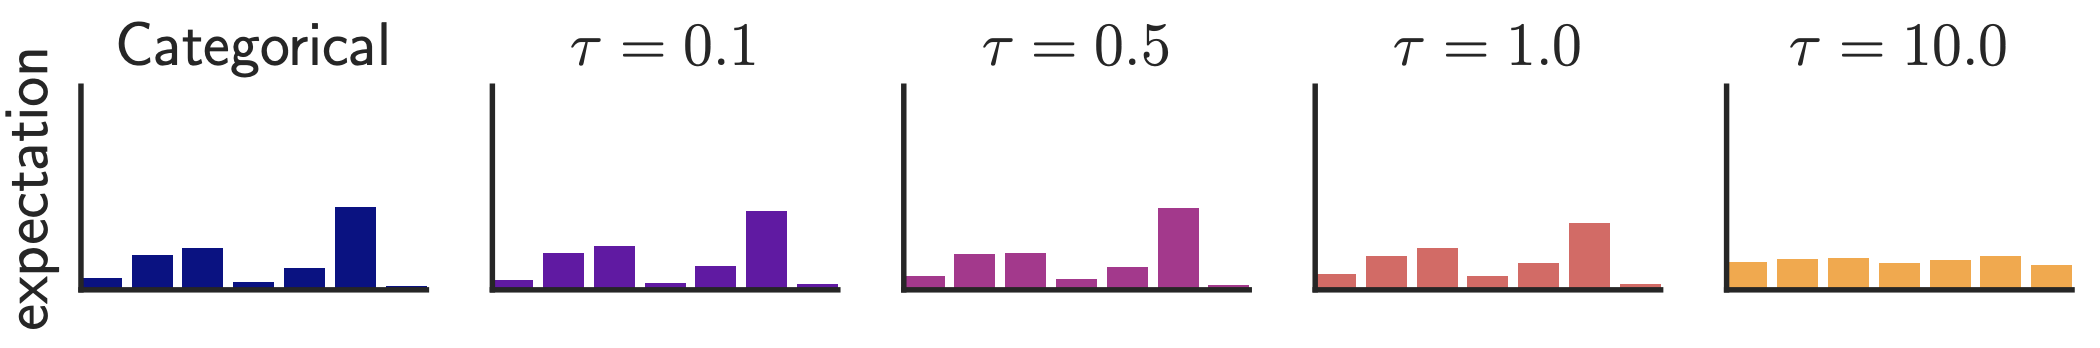
\includegraphics[width=0.8\linewidth]{figs/gumbel_softmax}
	 	\end{figure}
	 	\vspace{-0.7cm}
	 	\begin{figure}
	 		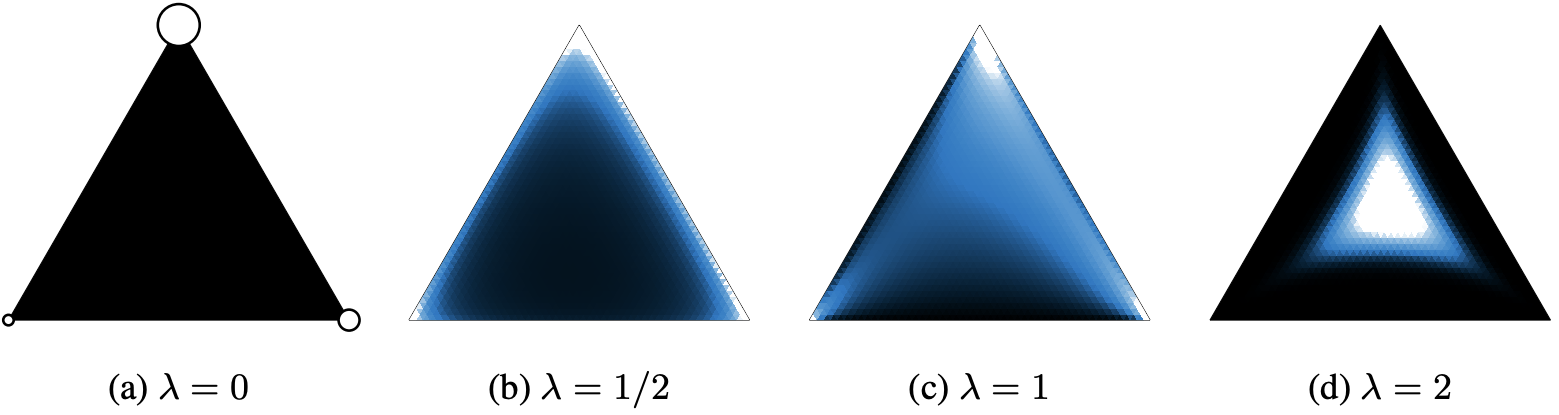
\includegraphics[width=0.8\linewidth]{figs/simplex}
	 	\end{figure} 
	 	\vspace{-0.5cm}
	 \end{block}
	\begin{block}{Reparametrization trick}
		\vspace{-0.4cm}
		\[
			\nabla_{\bphi} \mathbb{E}_{q(c | \bx, \bphi)} \log p(\bx | \be_{c} , \btheta) = \bbE_{\text{Gumbel}(0, 1)} \nabla_{\bphi} \log p(\bx | \bz , \btheta),
		\]
		where $\bz = \sum_{k=1}^K\hat{c}_k \be_k$ (all operations are differentiable now).
	\end{block}
 	\vspace{-0.2cm}
	\myfootnote{
	\href{https://arxiv.org/abs/1611.00712}{Maddison C. J., Mnih A., Teh Y. W. The Concrete distribution: A continuous relaxation of discrete random variables, 2016} \\
	\href{https://arxiv.org/abs/1611.01144}{Jang E., Gu S., Poole B. Categorical reparameterization with Gumbel-Softmax, 2016}
	}
\end{frame}
%=======
\begin{frame}{DALL-E/dVAE}
	\begin{block}{Deterministic VQ-VAE posterior}
		\vspace{-0.3cm}
		\[
			q(\hat{z}_{ij} = k^* | \bx) = \begin{cases}
				1 , \quad \text{for } k^* = \argmin_k \| [\bz_e]_{ij} - \be_k \| \\
				0, \quad \text{otherwise}.
			\end{cases}
		\]
		\vspace{-0.3cm}
	\end{block}
	\begin{itemize}
		\item Gumbel-Softmax trick allows to make true categorical distribution and sample from it.
		\item Since latent space is discrete we could train autoregressive transformers in it.
		\item It is a natural way to incorporate text and image token spaces.
	\end{itemize}
	\begin{figure}
		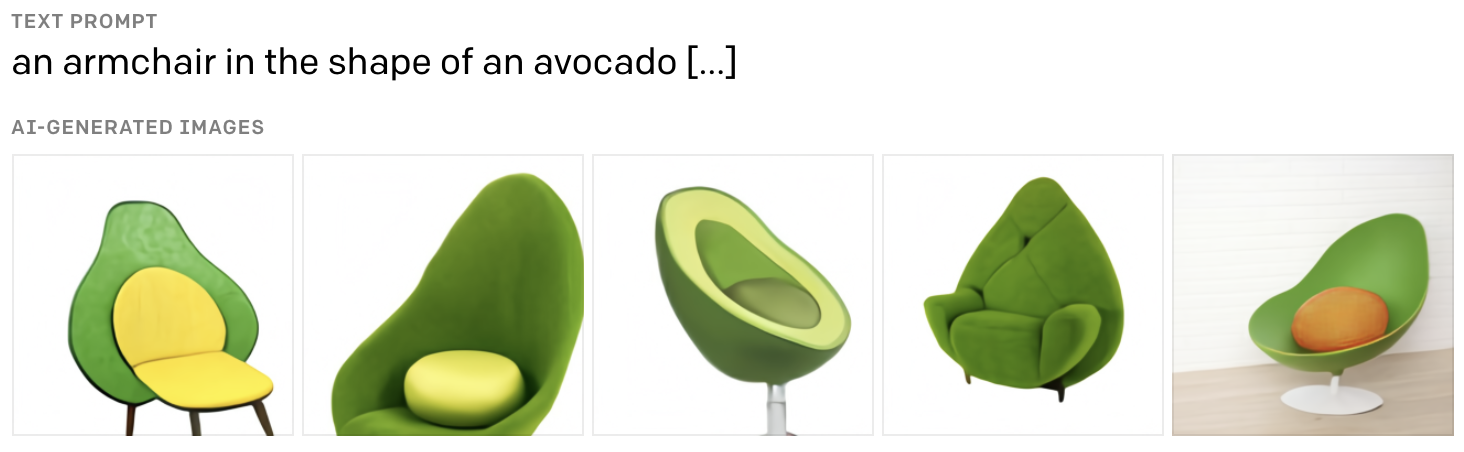
\includegraphics[width=\linewidth]{figs/dalle}
	\end{figure}
	\myfootnotewithlink{https://arxiv.org/abs/2102.1209}{Ramesh A. et al. Zero-shot text-to-image generation, 2021}
\end{frame}
%=======
\begin{frame}{Outline}
	\tableofcontents
\end{frame}
%=======
\section{ELBO surgery}
%=======
\begin{frame}{ELBO surgery}
	\vspace{-0.3cm}
	\[
	    \frac{1}{n} \sum_{i=1}^n \mathcal{L}_i(\bphi, \btheta) = \frac{1}{n} \sum_{i=1}^n \Bigl[ \mathbb{E}_{q(\bz | \bx_i, \bphi)} \log p(\bx_i | \bz, \btheta) - KL(q(\bz | \bx_i, \bphi) || p(\bz)) \Bigr].
	\]
	\vspace{-0.3cm}
	\begin{block}{Theorem}
		\vspace{-0.5cm}
		\[
		    \frac{1}{n} \sum_{i=1}^n KL(q(\bz | \bx_i, \bphi) || p(\bz)) = {\color{violet} KL(q_{\text{agg}}(\bz | \bphi) || p(\bz))} + {\color{teal}\bbI_{q} [\bx, \bz]};
		\]
		\vspace{-0.5cm}
		\begin{itemize}
			\item $q_{\text{agg}}(\bz | \bphi) = \frac{1}{n} \sum_{i=1}^n q(\bz | \bx_i, \bphi)$ -- \textbf{aggregated} posterior distribution.
			\item $\bbI_{q} [\bx, \bz]$ -- mutual information between $\bx$ and $\bz$ under empirical data distribution and distribution $q(\bz | \bx, \bphi)$.
			\item  {\color{violet} First term} pushes $q_{\text{agg}}(\bz | \bphi)$ towards the prior $p(\bz)$.
			\item {\color{teal}Second term} reduces the amount of	information about $\bx$ stored in $\bz$. 
		\end{itemize}
	\end{block}
	\myfootnotewithlink{http://approximateinference.org/accepted/HoffmanJohnson2016.pdf}{Hoffman M. D., Johnson M. J. ELBO surgery: yet another way to carve up the variational evidence lower bound, 2016}
\end{frame}
%=======
\begin{frame}{ELBO surgery}
		\vspace{-0.3cm}
		\[
		    \frac{1}{n} \sum_{i=1}^n KL(q(\bz | \bx_i, \bphi) || p(\bz)) = KL(q_{\text{agg}}(\bz | \bphi) || p(\bz)) + \bbI_q [\bx, \bz].
		\]
		\vspace{-0.3cm}
	\begin{block}{Proof}
		\vspace{-0.5cm}
		{\footnotesize
		\begin{multline*}
		    \frac{1}{n} \sum_{i=1}^n KL(q(\bz | \bx_i, \bphi) || p(\bz)) = \frac{1}{n} \sum_{i=1}^n \int q(\bz | \bx_i, \bphi) \log \frac{q(\bz | \bx_i, \bphi)}{p(\bz)} d \bz = \\
		    = \frac{1}{n} \sum_{i=1}^n \int q(\bz | \bx_i, \bphi) \log \frac{{\color{violet}q_{\text{agg}}(\bz | \bphi)} {\color{teal}q(\bz | \bx_i, \bphi)}}{{\color{violet}p(\bz)} {\color{teal}q_{\text{agg}}(\bz | \bphi)}} d \bz = \\
		    = \int \frac{1}{n} \sum_{i=1}^n  q(\bz | \bx_i, \bphi) \log {\color{violet}\frac{q_{\text{agg}}(\bz | \bphi)}{p(\bz)}} d \bz
		    + \frac{1}{n}\sum_{i=1}^n \int q(\bz | \bx_i, \bphi) \log {\color{teal}\frac{q(\bz | \bx_i, \bphi)}{q_{\text{agg}}(\bz | \bphi)}} d \bz = \\
		    = KL (q_{\text{agg}}(\bz | \bphi) || p(\bz)) + \frac{1}{n}\sum_{i=1}^n KL(q(\bz | \bx_i, \bphi) || q_{\text{agg}}(\bz | \bphi))
		\end{multline*}
		}
		\vspace{-0.4cm}
		\[
			\bbI_{q} [\bx, \bz] = \frac{1}{n}\sum_{i=1}^n KL(q(\bz | \bx_i, \bphi) || q_{\text{agg}}(\bz | \bphi)).
		\]
	\end{block}

	\myfootnotewithlink{http://approximateinference.org/accepted/HoffmanJohnson2016.pdf}{Hoffman M. D., Johnson M. J. ELBO surgery: yet another way to carve up the variational evidence lower bound, 2016}
\end{frame}
%=======
\begin{frame}{ELBO surgery}
	\begin{block}{ELBO revisiting}
		\vspace{-0.7cm}
		{\small
		\begin{multline*}
		    \frac{1}{n}\sum_{i=1}^n \cL_i(\bphi, \btheta) = \frac{1}{n} \sum_{i=1}^n \left[ \mathbb{E}_{q(\bz | \bx_i, \bphi)} \log p(\bx_i | \bz, \btheta) - KL(q(\bz | \bx_i, \bphi) || p(\bz)) \right] = \\
		    = \underbrace{\frac{1}{n} \sum_{i=1}^n \mathbb{E}_{q(\bz | \bx_i, \bphi)} \log p(\bx_i | \bz, \btheta)}_{\text{Reconstruction loss}} - \underbrace{\vphantom{ \sum_{i=1}^n} \bbI_q [\bx, \bz]}_{\text{MI}} - \underbrace{\vphantom{ \sum_{i=1}^n} KL(q_{\text{agg}}(\bz | \bphi) || {\color{teal}p(\bz)})}_{\text{Marginal KL}}
		\end{multline*}
		}
		\vspace{-0.3cm}
	\end{block}
	Prior distribution $p(\bz)$ is only in the last term.
	\begin{block}{Optimal VAE prior}
		\vspace{-0.7cm}
		\[
	  		KL(q_{\text{agg}}(\bz | \bphi) || p(\bz)) = 0 \quad \Leftrightarrow \quad p (\bz) = q_{\text{agg}}(\bz | \bphi) = \frac{1}{n} \sum_{i=1}^n q(\bz | \bx_i, \bphi).
		\]
		\vspace{-0.4cm} \\
		The optimal prior $p(\bz)$ is the aggregated posterior $q_{\text{agg}}(\bz | \bphi)$!
	\end{block}
	
	\myfootnotewithlink{http://approximateinference.org/accepted/HoffmanJohnson2016.pdf}{Hoffman M. D., Johnson M. J. ELBO surgery: yet another way to carve up the variational evidence lower bound, 2016}
\end{frame}
%=======
\begin{frame}{Variational posterior}
	\vspace{-0.3cm}
	\begin{block}{ELBO decomposition}
		\vspace{-0.3cm}
		\[
			\log p(\bx | \btheta) = \mathcal{L}(\bphi, \btheta) + KL(q(\bz | \bx, \bphi) || p(\bz | \bx, \btheta)).
		\]
		\vspace{-0.7cm}
	\end{block}
	\begin{itemize}
		\item $q(\bz | \bx, \bphi) = \mathcal{N}(\bmu_{\bphi}(\bx), \bsigma^2_{\bphi}(\bx))$ is a unimodal distribution. 
		\item The optimal prior $p(\bz)$ is the aggregated posterior $q_{\text{agg}}(\bz | \bphi)$.
	\end{itemize}
	
	\vspace{-0.3cm}
	\begin{figure}
		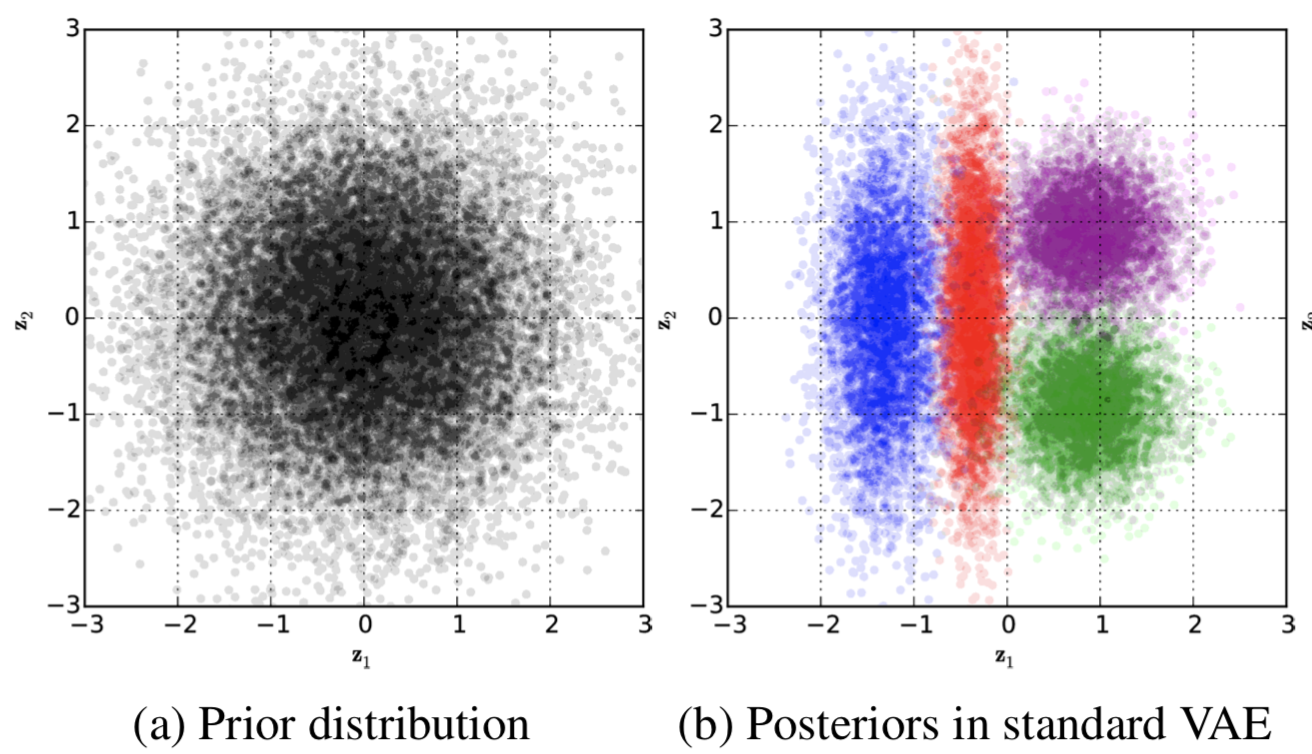
\includegraphics[width=0.65\linewidth]{figs/agg_posterior}
	\end{figure}
	\vspace{-0.3cm}
	It is widely believed that \textbf{mismatch between} $p(\bz)$  \textbf{and} $q_{\text{agg}}(\bz | \bphi)$  \textbf{is the main reason of blurry images of VAE}.
	\myfootnotewithlink{https://arxiv.org/abs/1505.05770}{Rezende D. J., Mohamed S. Variational Inference with Normalizing Flows, 2015} 
\end{frame}
%=======
\section{Learnable VAE prior}
%=======
\begin{frame}{Optimal VAE prior}
	\begin{itemize}
		\item Standard Gaussian $p(\bz) = \mathcal{N}(0, \bI)$ $\Rightarrow$ over-regularization;
		\item $p(\bz) = q_{\text{agg}}(\bz | \bphi) = \frac{1}{n}\sum_{i=1}^n q(\bz | \bx_i, \bphi)$ $\Rightarrow$ overfitting and highly expensive.
	\end{itemize}
	\vspace{-0.5cm}
	\begin{minipage}[t]{0.5\columnwidth}
		\begin{block}{Non learnable prior $p(\bz)$}
			\begin{figure}[h]
				\centering
				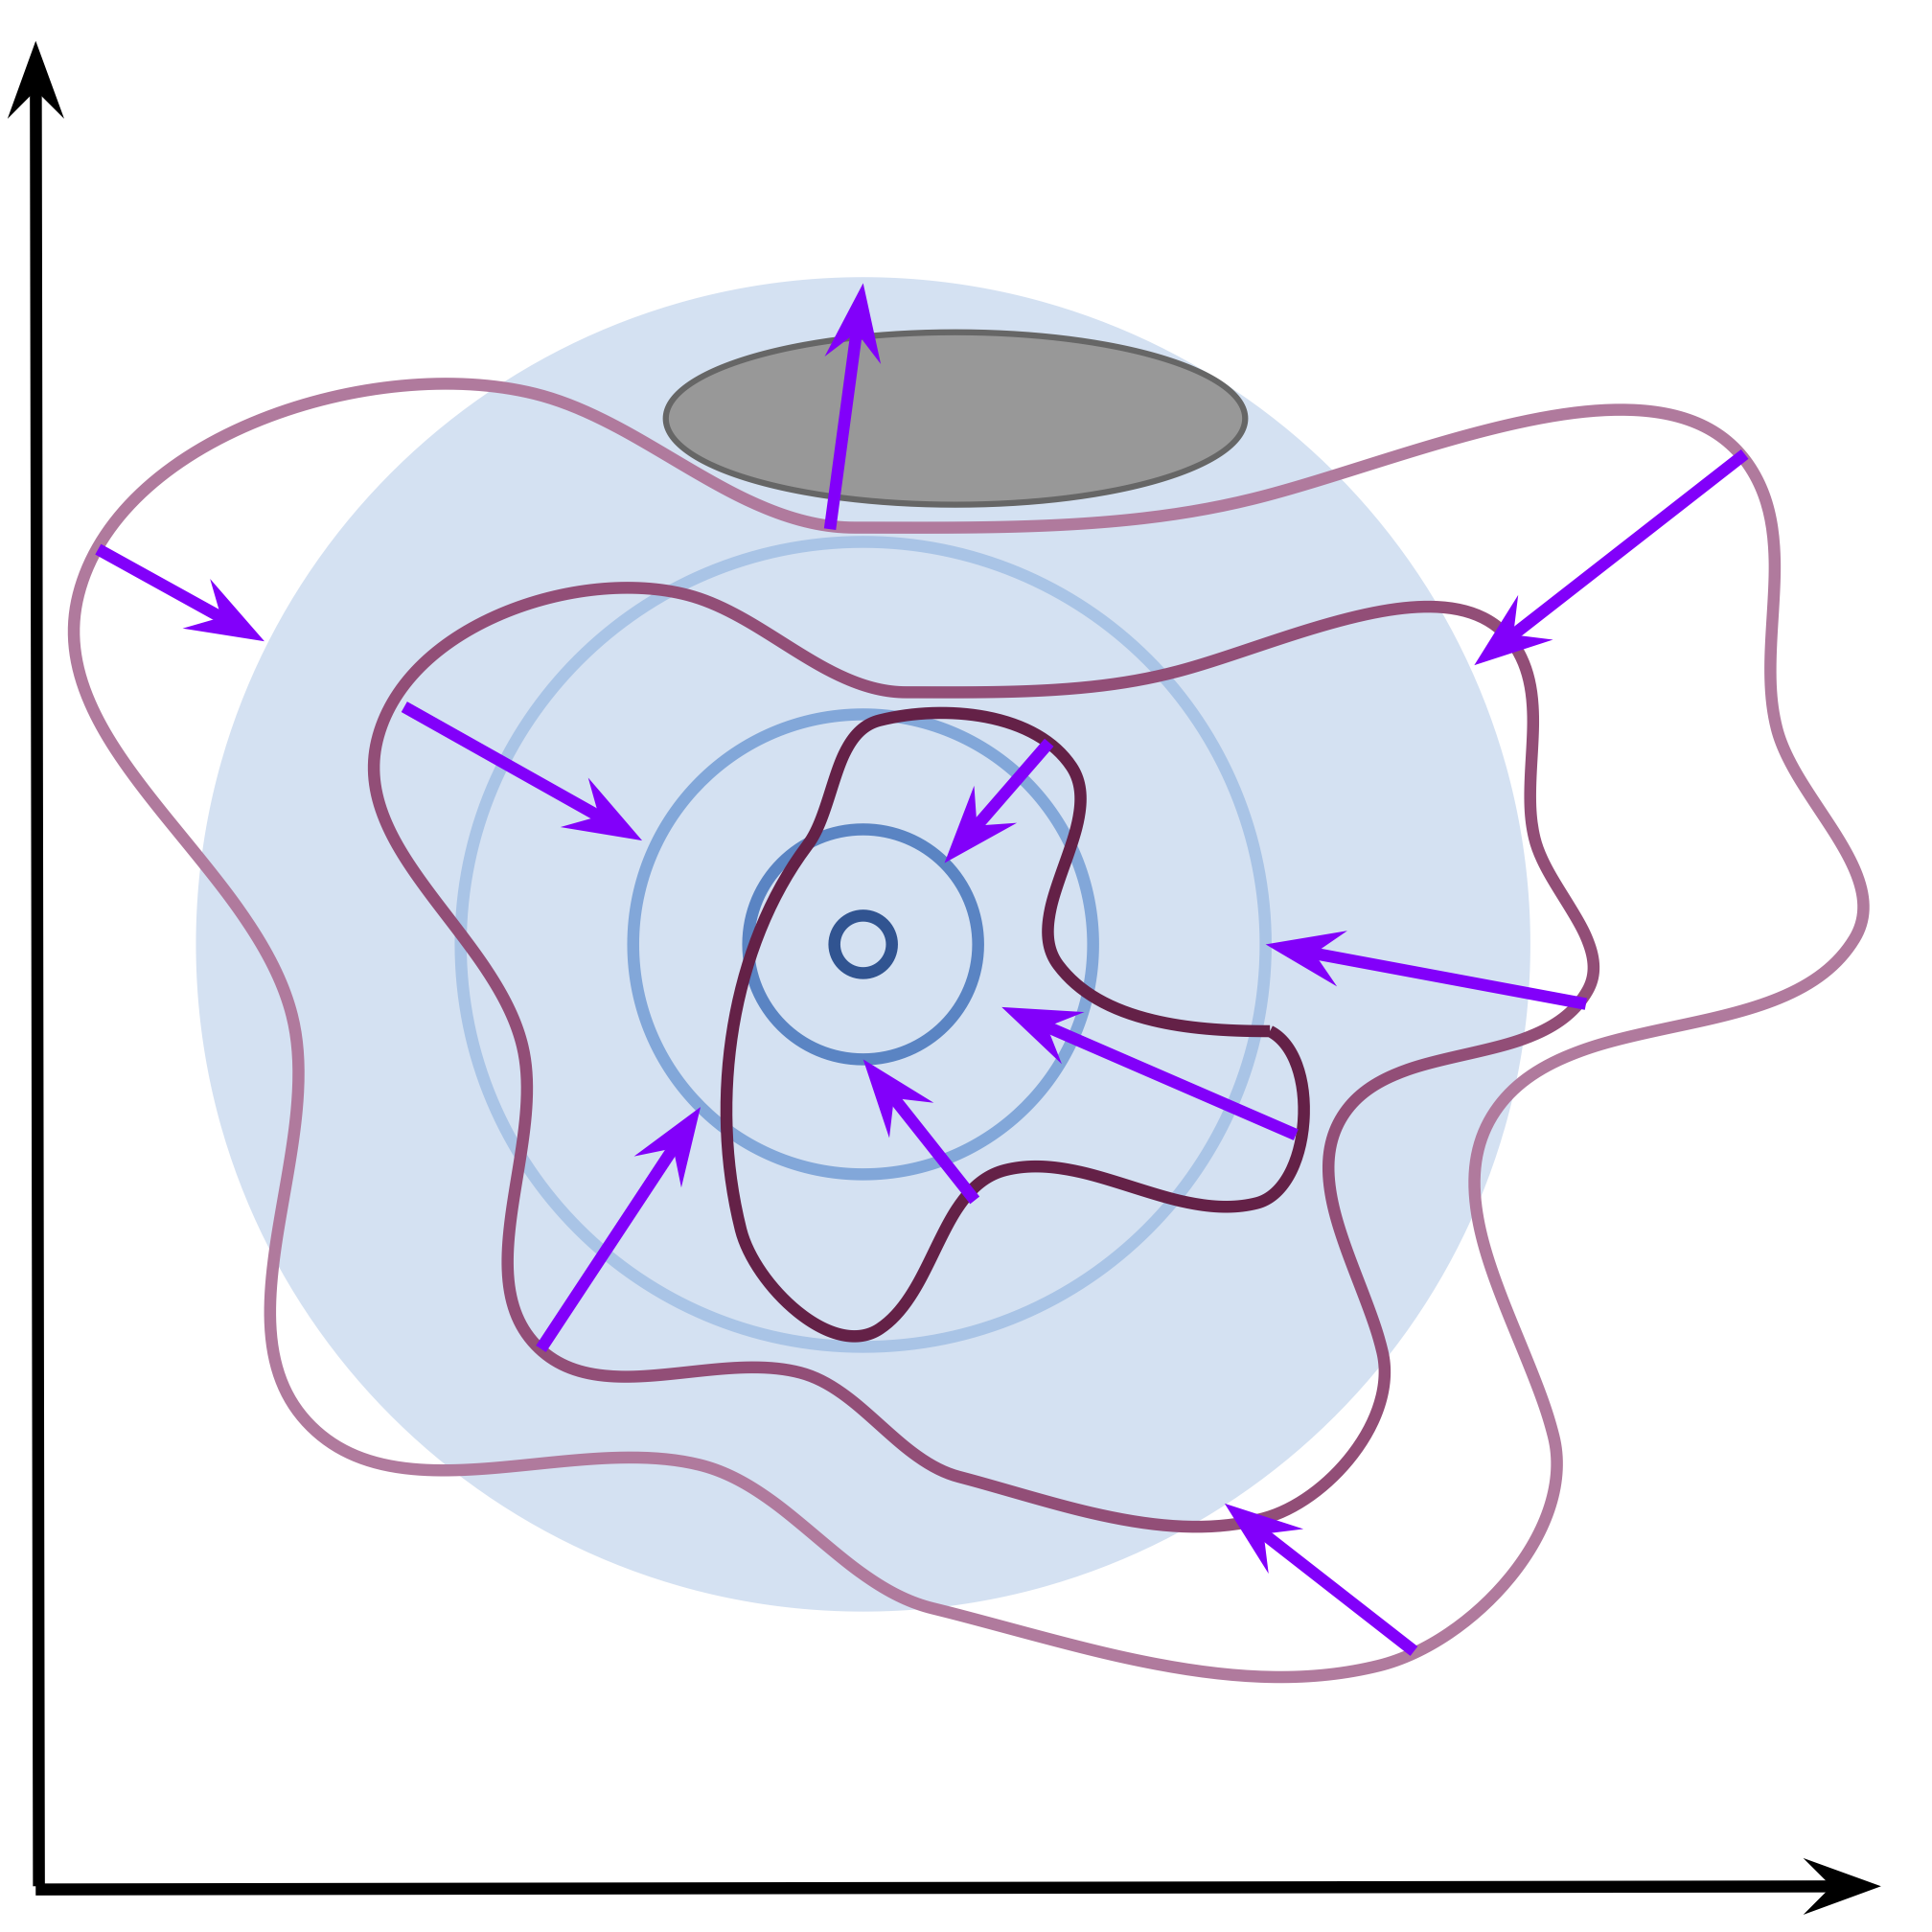
\includegraphics[width=0.6\linewidth]{figs/non_learnable_prior}
			\end{figure}
		\end{block}
	\end{minipage}%
	\begin{minipage}[t]{0.5\columnwidth}
		\begin{block}{Learnable prior $p(\bz | \blambda)$}
			\begin{figure}[h]
				\centering
				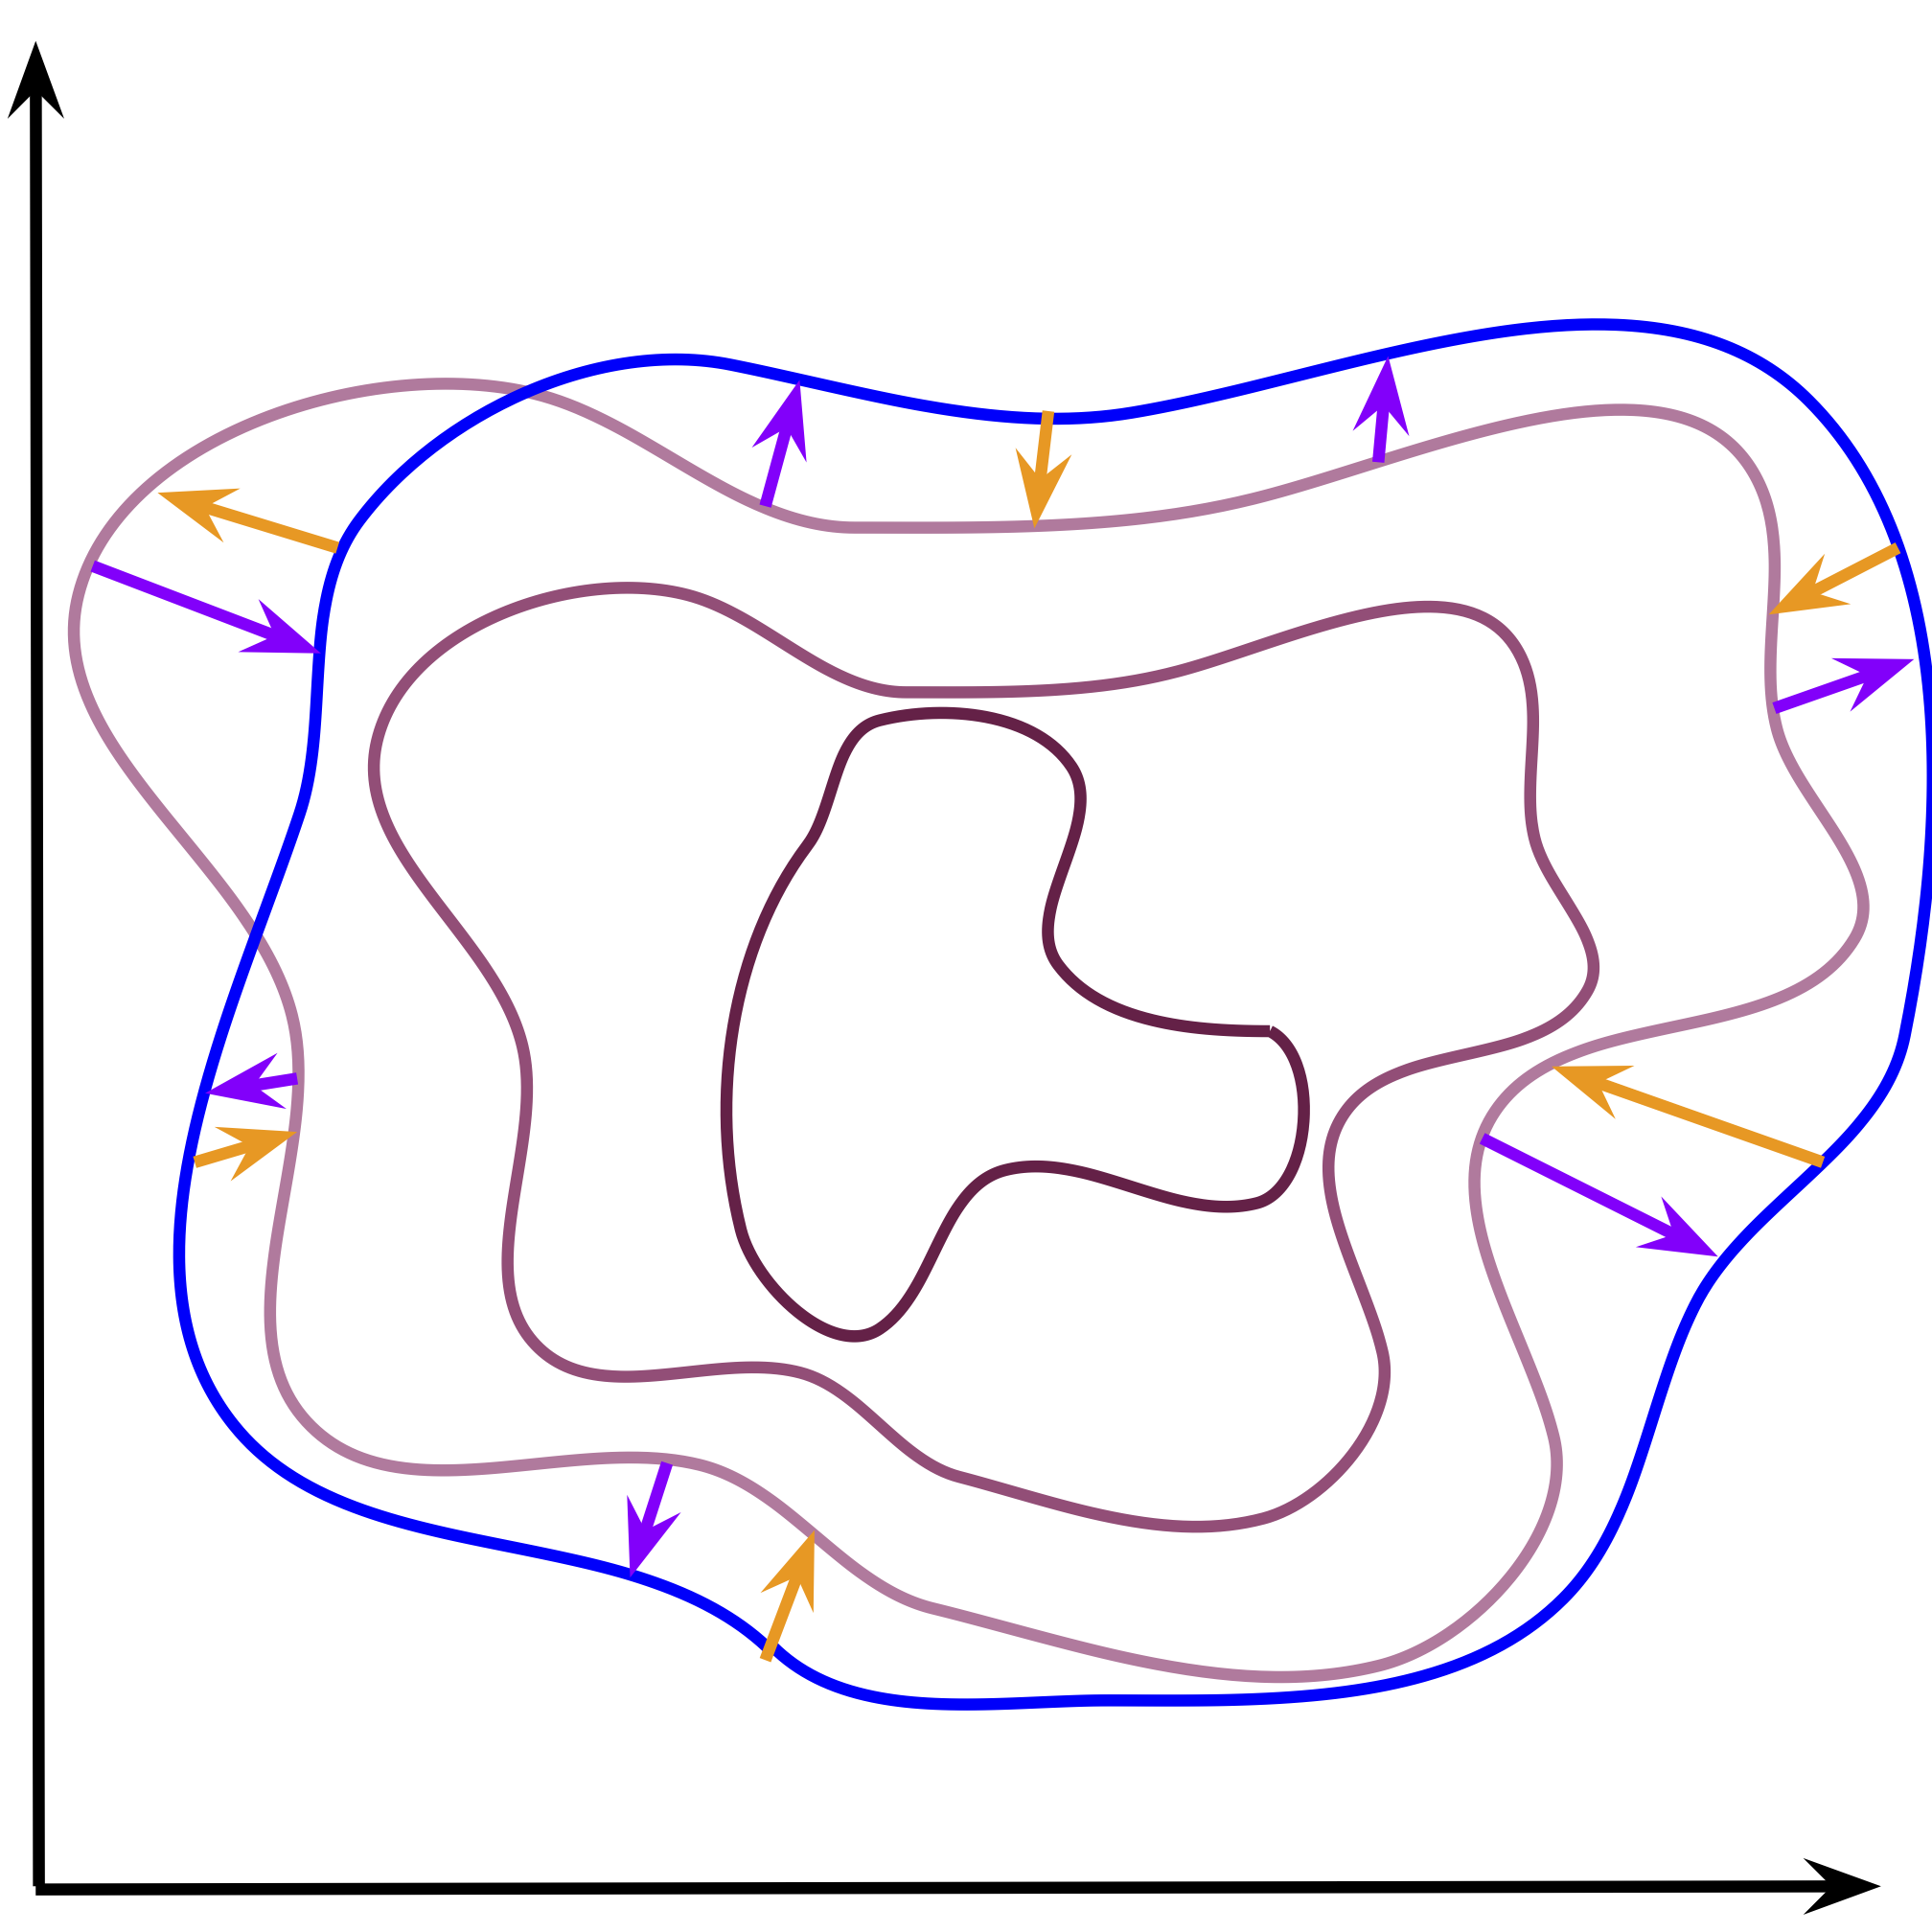
\includegraphics[width=0.6\linewidth]{figs/learnable_prior}
			\end{figure}
		\end{block}
	\end{minipage}
	\vspace{-0.4cm}
	\begin{block}{ELBO revisiting}
		\vspace{-0.3cm}
		\[
			\frac{1}{n}\sum_{i=1}^n \cL_i(\bphi, \btheta) = \text{RL} - \text{MI} -  KL(q_{\text{agg}}(\bz | \bphi) || {\color{teal}p(\bz | \blambda)})
		\]
		It is Forward KL with respect to $p(\bz | \blambda)$.
	\end{block}
	\myfootnotewithlink{https://jmtomczak.github.io/blog/7/7\_priors.html}{image credit: https://jmtomczak.github.io/blog/7/7\_priors.html}
\end{frame}
%=======
\begin{frame}{NF-based VAE prior}
	\begin{block}{NF model in latent space}
		\vspace{-0.5cm}
		\[
			\log p(\bz | \blambda) = \log p(\bz^*) + \log  \left | \det \left(\frac{d \bz^*}{d\bz}\right)\right| = \log p(\bff_{\blambda}(\bz)) + \log \left | \det (\bJ_\bff)\right| 
		\]
		\vspace{-0.3cm}
		\[
			\bz = \bg_{\blambda}(\bz^*) = \bff^{-1}_{\blambda}(\bz^*)
		\]
	\end{block}
	\vspace{-0.3cm}
	\begin{itemize}
		\item RealNVP with coupling layers.
		\item Autoregressive NF (fast $\bff_{\blambda}(\bz)$, slow $\bg_{\blambda}(\bz^*)$).
	\end{itemize}
	\begin{block}{ELBO with NF-based VAE prior}
		\vspace{-0.5cm}
		{\small
		\begin{multline*}
			\mathcal{L}(\bphi, \btheta) = \mathbb{E}_{q(\bz | \bx, \bphi)} \left[ \log p(\bx | \bz, \btheta) + {\color{violet}\log p(\bz | \blambda)} - \log q(\bz | \bx, \bphi) \right] \\
				= \mathbb{E}_{q(\bz | \bx, \bphi)} \Bigl[ \log p(\bx | \bz, \btheta) + \underbrace{ \Bigl({\color{violet} \log p(\bff_{\blambda}(\bz)) + \log \left| \det (\bJ_\bff) \right|} \Bigr) }_{\text{NF-based prior}} - \log q(\bz | \bx, \bphi) \Bigr] 
		\end{multline*}
		}
	\end{block}
	\myfootnotewithlink{https://arxiv.org/abs/1611.02731}{Chen X. et al. Variational Lossy Autoencoder, 2016}
\end{frame}
%=======
\begin{frame}{Summary}
	\begin{itemize}
		\item The ELBO surgery reveals insights about a prior distribution in VAE. The optimal prior is the aggregated posterior. It is widely believed that mismatch between $p(\bz)$ and $q_{\text{agg}}(\bz | \bphi)$ is the main reason of blurry images of VAE.
		\vfill
		\item We could use NF-based prior in VAE (even autoregressive).
		\vfill	
		\item Vector Quantization is the way to create VAE with discrete latent space and deterministic variational posterior. 
		\vfill
		\item Straight-through gradient ignores quantize operation in backprop.			
		\vfill
		\item Gumbel-softmax trick relaxes discrete problem to continuous one using Gumbel-max reparametrization trick.
	\end{itemize}
\end{frame}

\end{document} 
